\documentclass{beamer}
\usetheme{Madrid}

\usepackage[utf8]{inputenc}
\usepackage{subfig}
\usepackage{tikz}   
\usepackage{hyperref}
\hypersetup{
    colorlinks=false,
    citecolor=black,
    filecolor=magenta,      
    urlcolor=cyan,
}
\captionsetup[subfloat]{labelformat=empty}

% \usepackage{biblatex}
\usepackage[
backend=biber,
style=numeric,
% citestyle=numeric
bibstyle=ieee
]{biblatex}

\addbibresource{bibl.bib} %Imports bibliography file

\title[FGNs vs Adversarial Attacks] %optional
{Finite Gaussian Neurons}
\subtitle{A Defense Against Adversarial Attacks?}

\author[Felix Grezes] % (optional, for multiple authors)
{Felix Grezes}

\institute[CUNY GC] % (optional)
{
  \inst{}%
  Graduate Center\\
  City University of New York
}

\date[Thesis Proposal - Spring 2021] % (optional)
{Thesis Proposal Fall 2021}

\logo{
\includegraphics[height=1.5cm]{images/gc_logo_286_3_300px_511px.png}}

\begin{document}

\frame{\titlepage}

\begin{frame}
    \frametitle{Table of Contents}
    \tableofcontents
\end{frame}


\section{Abstract}
\begin{frame}{Abstract}
Artificial neural networks have been shown to be vulnerable to adversarial attacks, which can imperceptibly alter inputs to fool the network into making wrong or nonsensical predictions.\\
\vspace{2mm}
In this work I introduce the Finite Gaussian Neuron, a novel neuron architecture for artificial neural networks.\\
\vspace{2mm}

My works aims to:
\begin{itemize}
    \item make it easy to convert existing models to the FGN architecture,
    \item while preserving the existing model's behavior on real data,
    \item and offering resistance against some adversarial attacks.
\end{itemize}

\end{frame}


\section{Introduction }
% \subsection{Definitions}
\begin{frame}{Introduction - Definitions}
    \begin{columns}
    \begin{column}{.29\textwidth}
    \vspace*{-4mm}
    \begin{figure}
        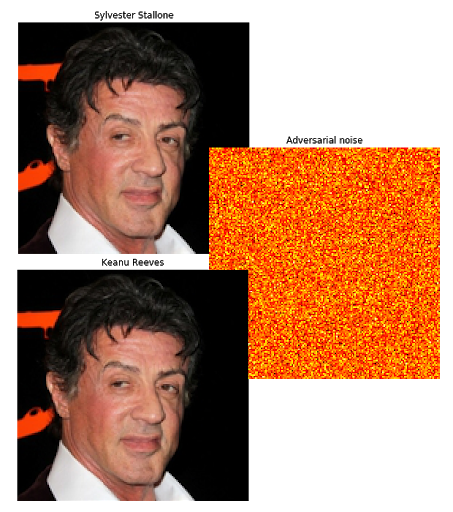
\includegraphics[width=1.\textwidth]{images/Definitions-examples/sly_ex.png}
    \end{figure}
    \vspace{-6mm}
    \centering{\tiny{ A Successful Attack (\cite{Mikhailov2017How} \href{https://blog.ycombinator.com/how-adversarial-attacks-work/}{Mikhailov}) }}
    \vspace{-1mm}
    \begin{figure}
        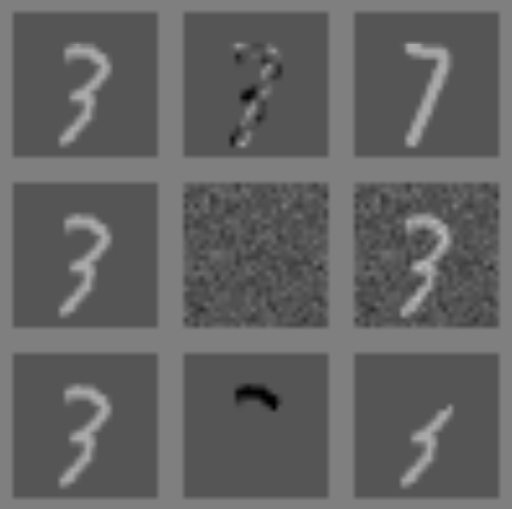
\includegraphics[width=.93\textwidth]{images/Definitions-examples/uninteresting attacks.png}
    \end{figure}
    \vspace{-6mm}
    \centering{\tiny{Uninteresting Attacks}}
    \end{column}
    
    \begin{column}{.55\textwidth}
        \vspace{-10mm}
        \begin{block}{Adversarial Examples}
            $\bullet$ An input to a trained model specifically designed to fool the model.\\
        \end{block}
    
        \begin{block}{Adversarial Attack}
            $\bullet$ A method of generating adversarial examples.\\
        \end{block}
        
        \begin{block}{Successful Attack Metrics}
            $\bullet$ confidence $\bullet$ distortion $\bullet$ un/targeted\\
             $\bullet$ white/blackbox $\bullet$ universal/tailored
        \end{block}
    \end{column}
    \end{columns}
    
\end{frame}
% \subsection{Motivation}
\begin{frame}{Introduction - Motivation}
    \centering \emph{Why are neural networks susceptible to adversarial attacks?}

    \begin{block}{Theory}
    A combination of the artificial neuron's \textbf{piece-wise linearity} combined with the \textbf{curse of dimensionality}, leading to:
    \begin{itemize}
        \item excessive confidence and generalization far from the training data,
        \item and inputs being close to the predicted borders with other classes.
    \end{itemize}
    \end{block}
    
    \begin{columns}
    \begin{column}{.34\textwidth}
    \begin{figure}
        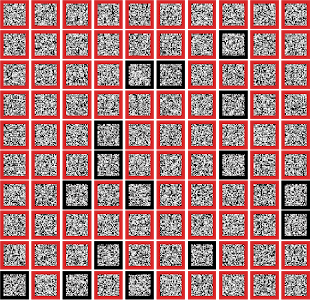
\includegraphics[width=.8\textwidth]{images/Motivation/pred_noise.png}
        \caption*{Predictions over white noise}
    \end{figure}
    \end{column}
    \begin{column}{.34\textwidth}
    \begin{figure}
        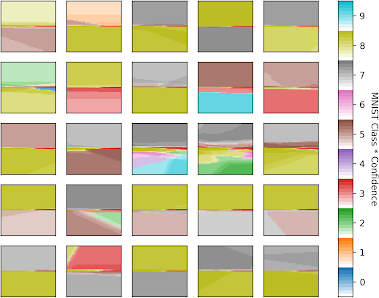
\includegraphics[width=1.\textwidth]{images/Motivation/boundaries.png}
        \caption*{Class boundaries on MNIST}
    \end{figure}
    \end{column}
    \end{columns}
    
\end{frame}

% \subsection{Related Work}
\begin{frame}{Related Work - Fast Gradient Sign Method}
    \begin{block}{}
    For each input dimension, take one fixed-size step in the direction of the gradient of the loss with regards to the input.
    \end{block}

   \begin{figure} 
       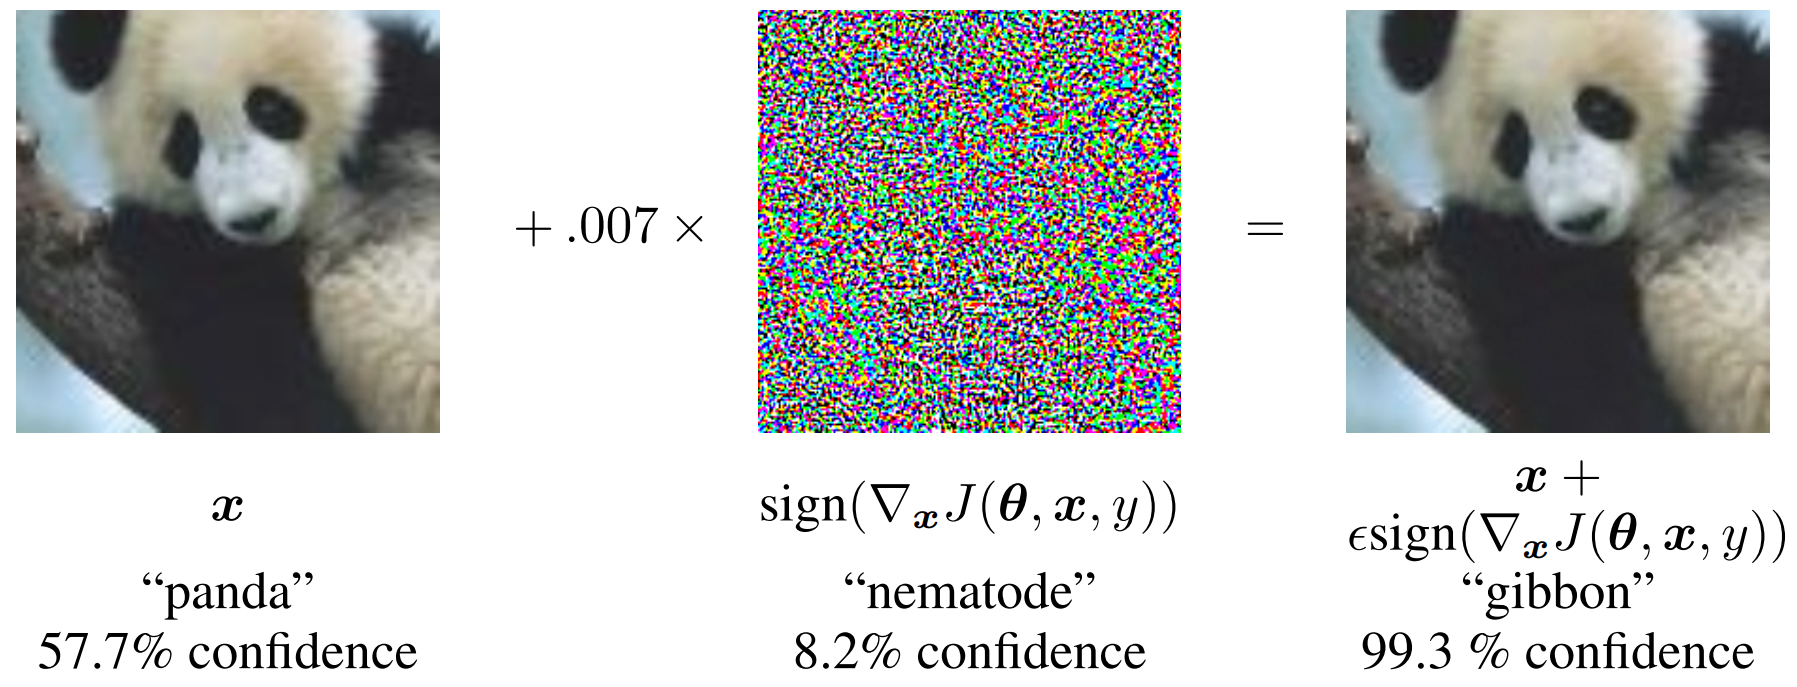
\includegraphics[width=0.9\textwidth]{images/Related-Work/FGSM-Example.PNG}
       \caption*{\cite{goodfellow2015explaining} \fullcite{goodfellow2015explaining}}
   \end{figure}
\end{frame}

\begin{frame}{Related Work - Adversarial Training}
    \begin{block}{Train on Adversarial Examples from Multi-step Gradient-based Attack }
        $\bullet$ Pros: potential universal robustness (vs first-order methods) \\
        $\bullet$ Cons: requires larger networks, generating examples, and retraining 
    \end{block}
    
   \begin{figure} 
       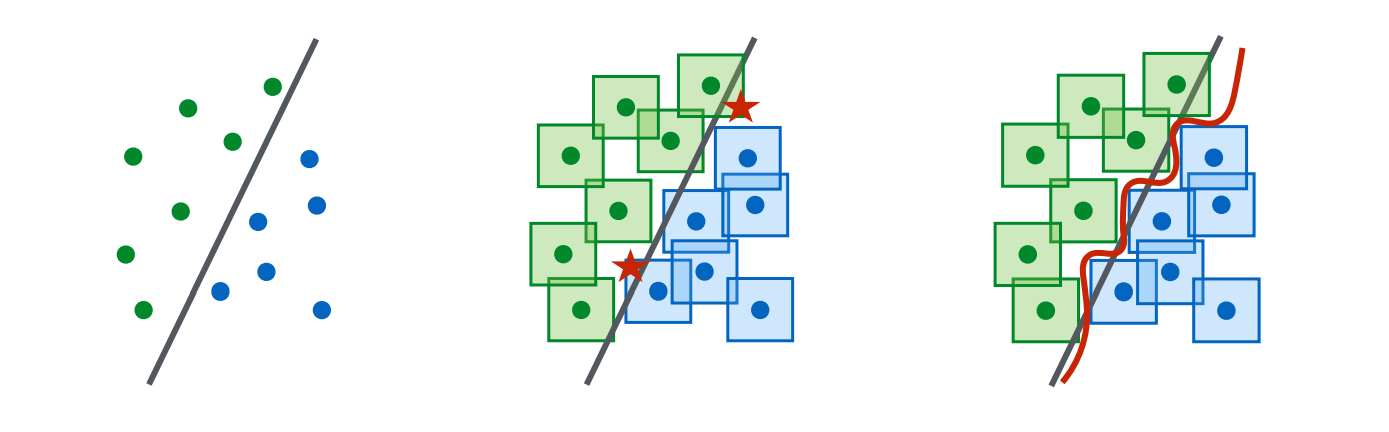
\includegraphics[width=0.9\textwidth]{images/Related-Work/adversarial-training.PNG}
       \caption*{\cite{madry2019deep} \fullcite{madry2019deep}}
   \end{figure}
    
\end{frame}

\begin{frame}{Related Work - Distillation}

    \begin{block}{Retrain on Output Predictions Vectors}
        $\bullet$ Pros: defends against attacks by reducing input sensitivity.\\
        $\bullet$ Cons: requires generating class probabilities, retraining.
    \end{block}

    
   \begin{figure} 
       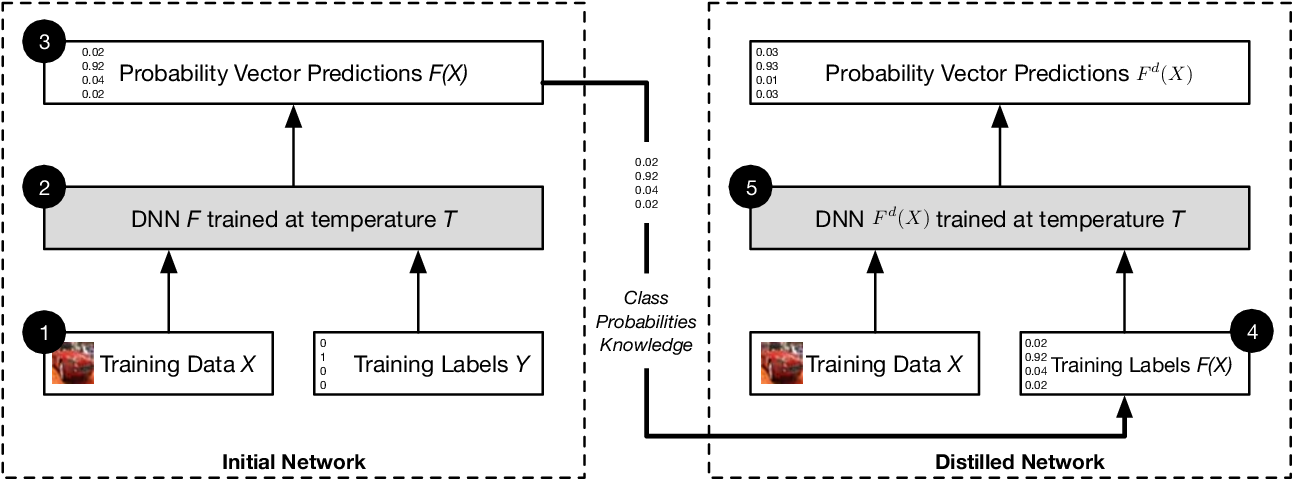
\includegraphics[width=0.8\textwidth]{images/Related-Work/distillation.png}
       \caption*{\cite{Papernot2016DistillationAA} \fullcite{Papernot2016DistillationAA}}
   \end{figure}
    
\end{frame}

\begin{frame}{Related Work - Radial Basis Function Networks}
    \begin{block}{}
        $\bullet$ Pros: Naturally resistant to rubbish and adversarial examples\\
        $\bullet$ Cons: Single layer, prototype pre-training
    \end{block}
    
    \begin{figure} 
    \begin{columns}
    \begin{column}{.49\textwidth}
       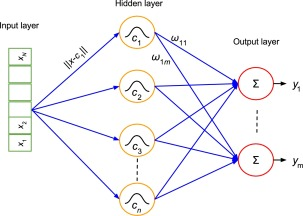
\includegraphics[width=0.99\textwidth]{images/Related-Work/RBF-net-low-qual.jpg}
    \end{column}
    
    \begin{column}{.49\textwidth}
        \begin{align*}
        \phi_i(x) &= \exp (-\frac{||x-c_i||^2}{2\sigma_i^2})\\
        y_k &= \sum_{i=1}^n w_{jk}\phi_i(x)
        \end{align*}
    \end{column}
    \end{columns}
    \caption*{\cite{samui2017handbook} \fullcite{samui2017handbook}\\
    \cite{chenou2019radial} \fullcite{chenou2019radial}}
    \end{figure} 

\end{frame}

% \begin{frame}{Related Work - Bayesian Neural Networks}
% % Q: BNNs can also answer "i don't know". How do FGNs differ?
% % Ensembles are not resistant to adversarial examples.
% \end{frame}

% \begin{frame}{Recent Advances: }
    
% \end{frame}



\section{The Finite Gaussian Neuron}

\begin{frame}{The Classical Neuron}
    % Classic neuron math
    \begin{block}{Neuron Output}
        \vspace{-1.5mm}
        $$y = \varphi(\ell)$$
    \end{block}
    \begin{block}{Linear Component}
        $$\ell=\sum_i x_i w_i$$
    \end{block}
    % classic neuron illustrated
    \begin{center}
        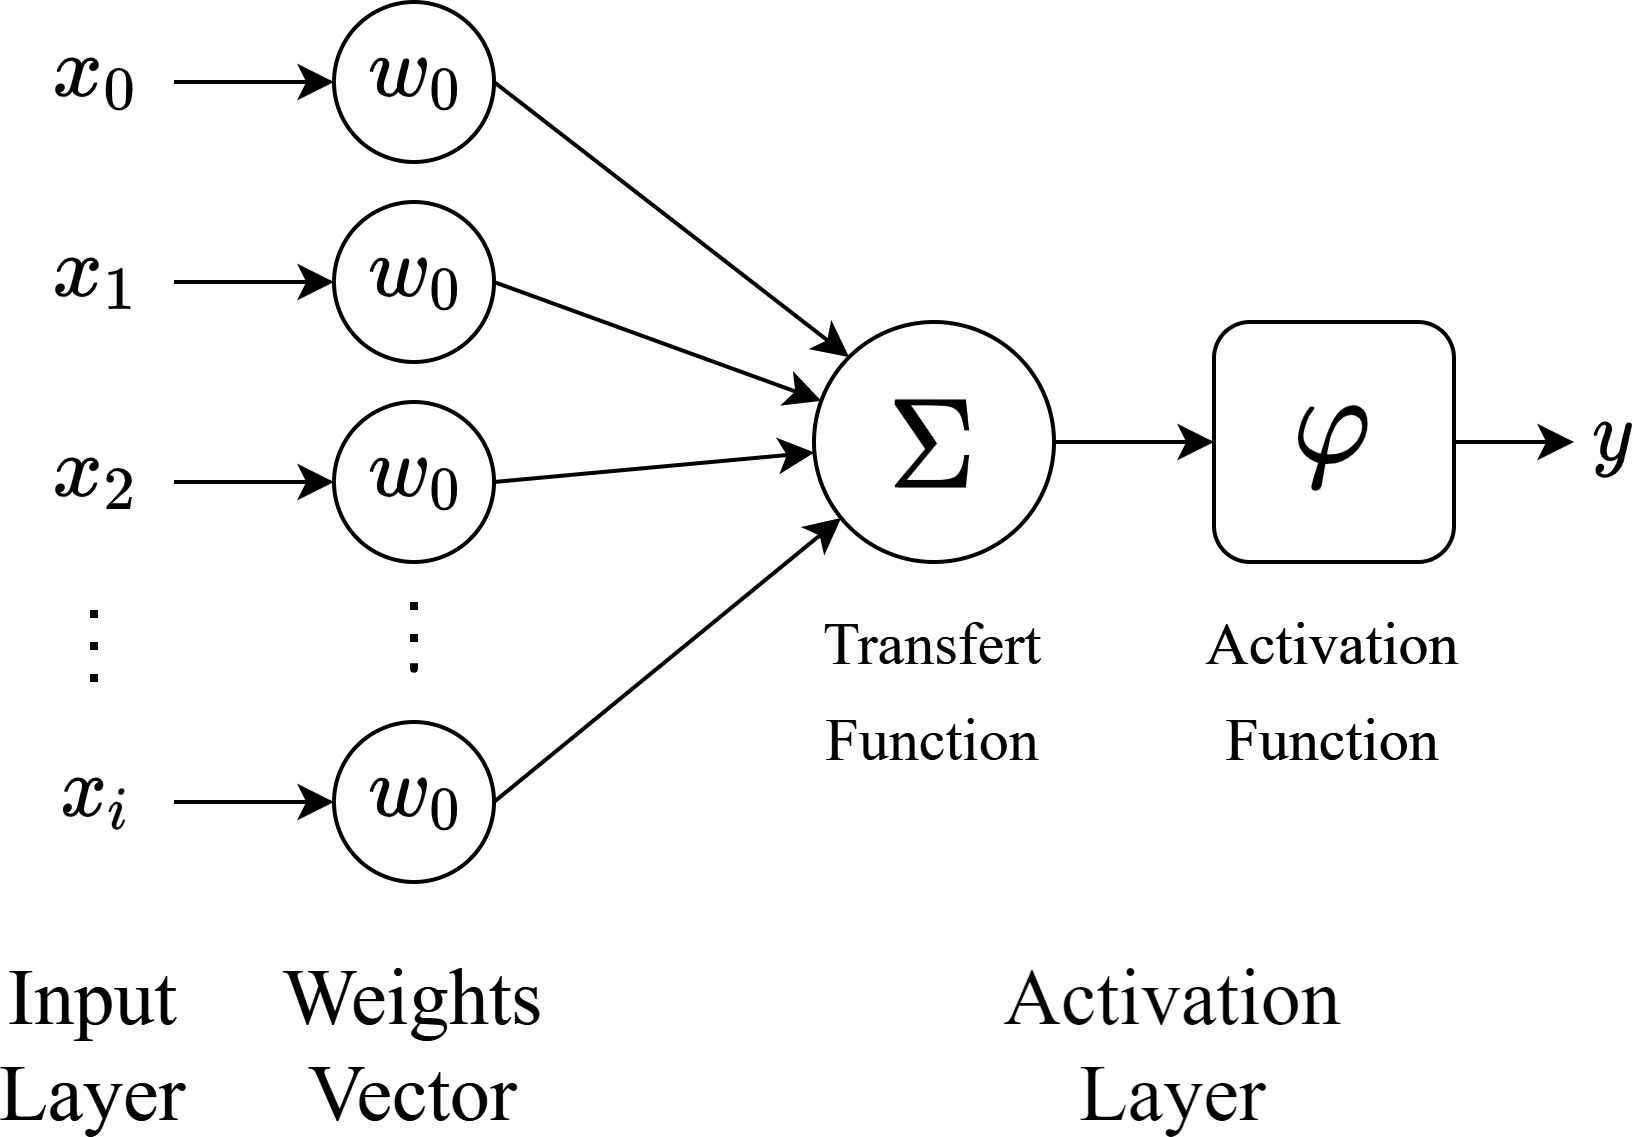
\includegraphics[width=0.5\textwidth]{images/classic-neuron.png}
    \end{center}
\end{frame}

\begin{frame}{The Finite Gaussian Neuron}
    %%math
    \begin{block}{Neuron Output}
        $$ y =  \varphi(\ell)*g = \varphi(\sum_i x_i w_i) * g$$
    \end{block}
    \begin{block}{Gaussian Component}
    % $$ g = exp \left( \frac{-1}{\sigma^2}*\sum_{i}(x_i-c_i)^2 \right)$$
    % $$ g = exp(\frac{-\sum_i (x_i-c_i)^2}{\sigma^2} )$$
    $$ g = e^{\frac{-1}{\sigma^2}\sum_{i}(x_i-c_i)^2}$$
    \end{block}
    %% gaussian component illustrated
    \begin{center}
        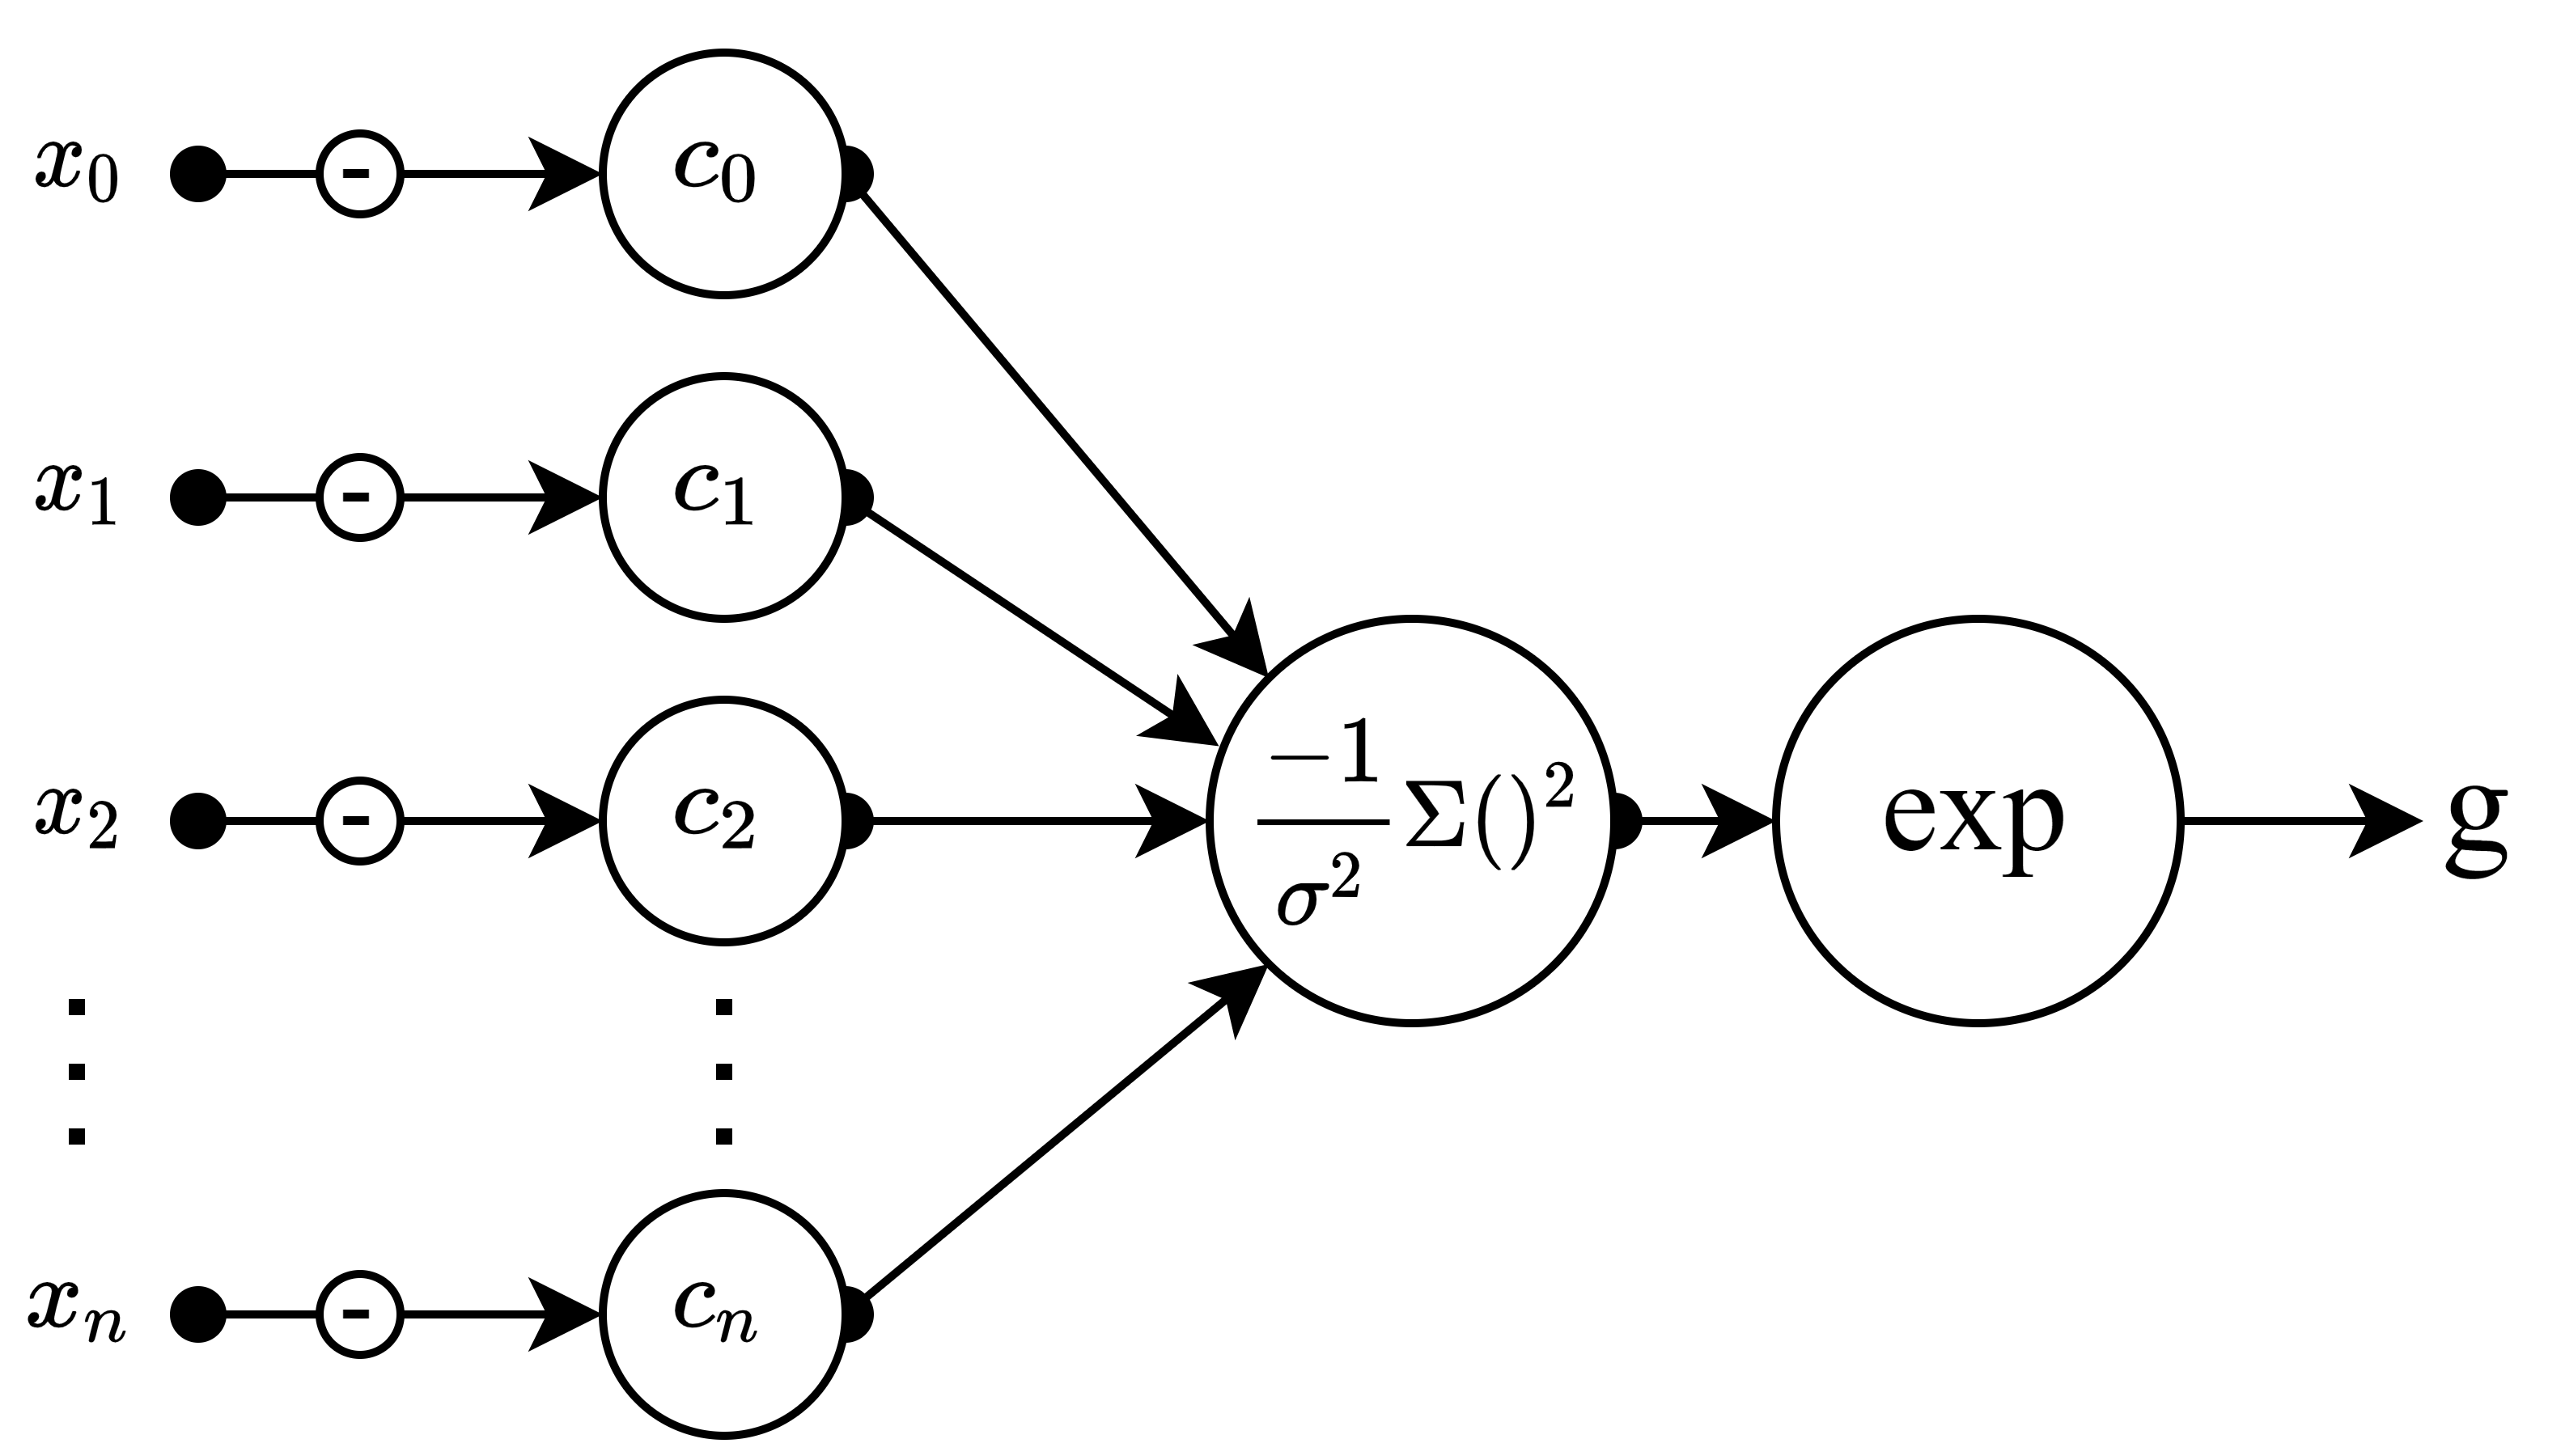
\includegraphics[width=0.5\textwidth]{images/fgn-gaussian-component.png}
    \end{center}
\end{frame}

\begin{frame}{2D Neuron Activity Visualization}
    % 2 images for classic: linear and after non-linearity like tanh
    % 2 images for fgn: gaussian component and combination 
    \vspace{-0.5cm}
    \begin{figure}
      \subfloat[Linear: $\ell = W^tX$]{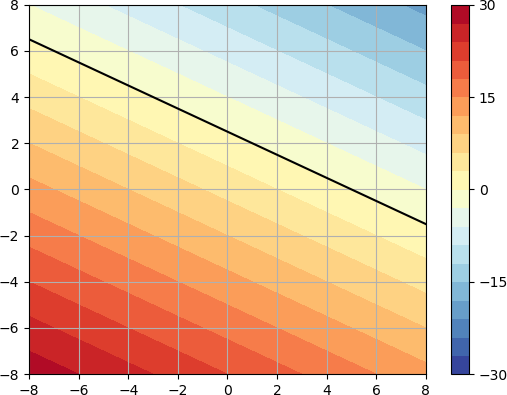
\includegraphics[height=3.2cm,width=4cm]{images/2D Activity/2d-linear-activity-cropped.png}} \hspace{0.5cm}
      \subfloat[Classic: $y = \tanh(\ell)$]{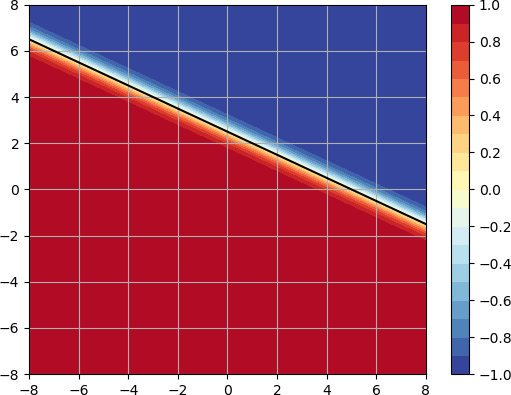
\includegraphics[height=3.2cm,width=4cm]{images/2D Activity/2d-classic-activity-cropped.png}}\\
      \vspace{-0.2cm}
      \subfloat[$g = e^{\frac{-1}{\sigma^2}*\sum_{i}(x_i-c_i)^2}$]{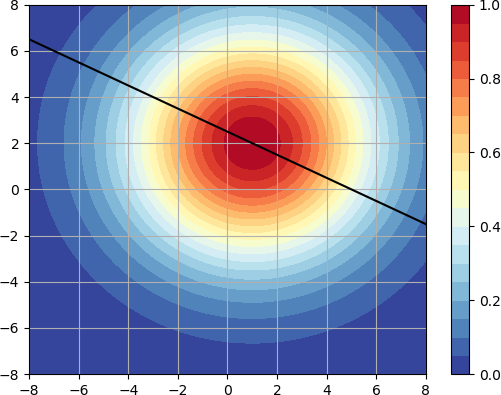
\includegraphics[height=3.2cm,width=4cm]{images/2D Activity/2d-gaussian-activity-cropped.png}} \hspace{0.5cm}
      \subfloat[FGN: $y = \tanh(\ell)*g$]{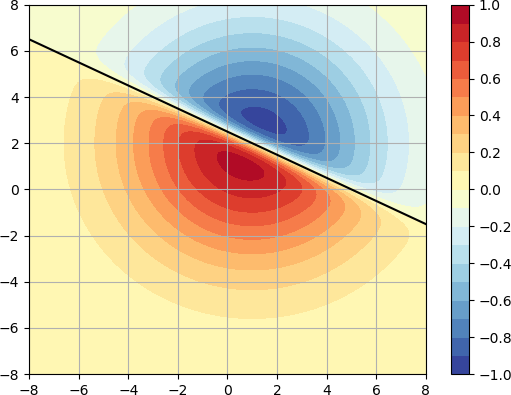
\includegraphics[height=3.2cm,width=4cm]{images/2D Activity/2d-fgn-activity-cropped.png}}
    \end{figure}
\end{frame}

\begin{frame}{Bird's Eye View - Desired Behavior}
    % \begin{figure}
    %     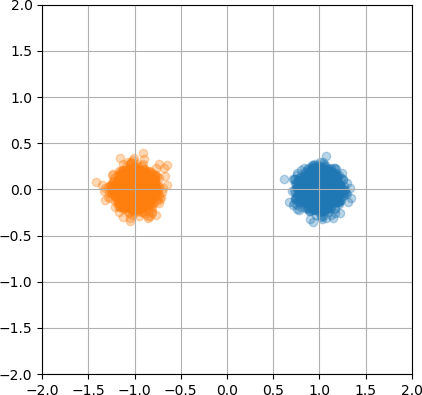
\includegraphics[width=.25\textwidth]{images/Bird's Eye View/data.png}
    % \end{figure}
    
    \begin{block}{Desired Behavior}
    $\bullet$ Restrict network activity to space that contains data.
    \end{block}
    
    \begin{columns}
    \begin{column}{.45\textwidth}
    \begin{figure}
        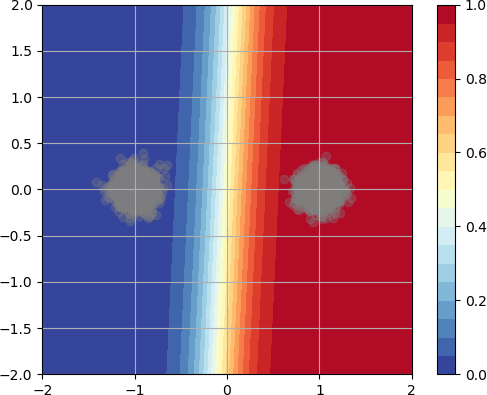
\includegraphics[width=\textwidth]{images/Bird's Eye View/classic_with_data.png}
        \caption*{Classic Network Behavior}
    \end{figure}
    \end{column}
    \begin{column}{.45\textwidth}
    \begin{figure}
        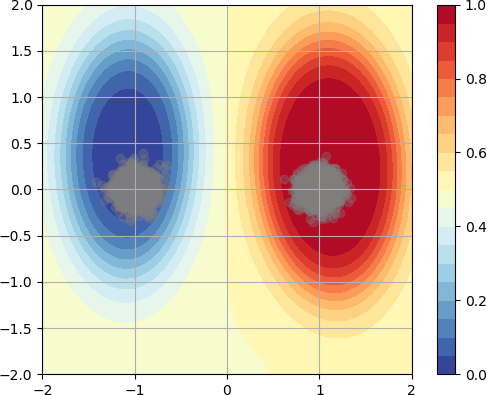
\includegraphics[width=\textwidth]{images/Bird's Eye View/fgn_with_data.png}
        \caption*{Desired FGN Network Behavior}
    \end{figure}
    \end{column}
    \end{columns}
    
\end{frame}


\begin{frame}{Matching Classical Neuron Behavior}
    \begin{block}{Property}
    As the neuron variance $\sigma$ increases, the Finite Gaussian Neuron's behavior gets closer that of the classical neuron with the same $W$ weights.
    \end{block}
    \vspace{0.2cm}
    \begin{tikzpicture}
        \node (img1) {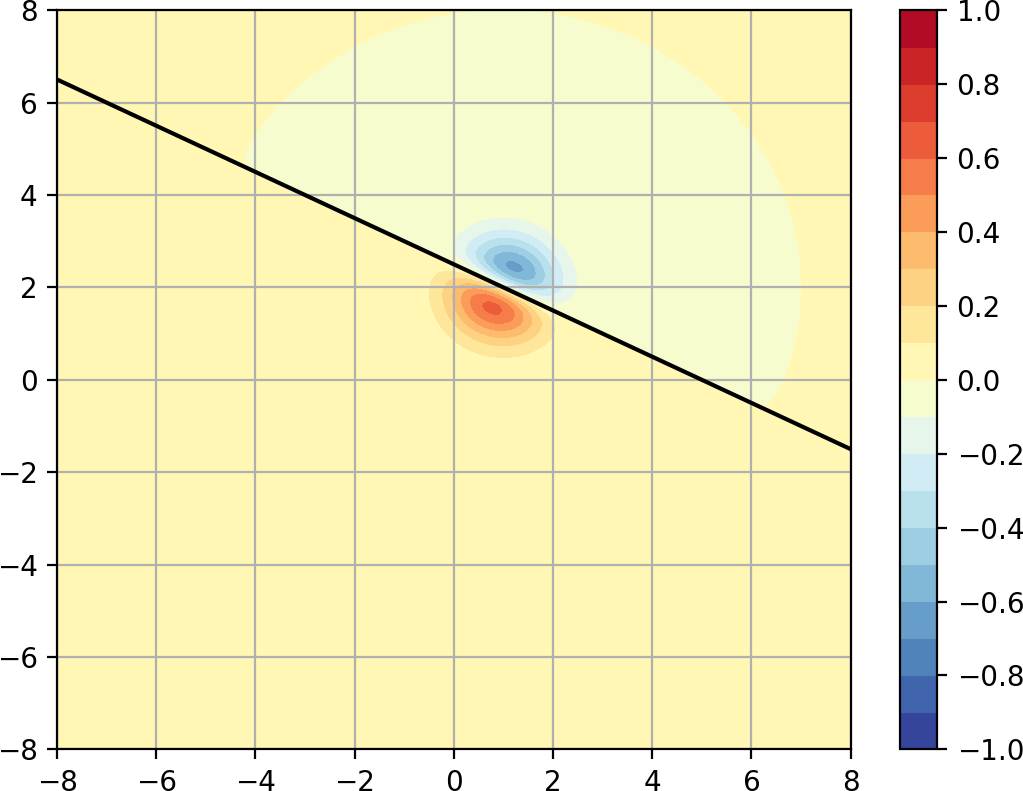
\includegraphics[height=3cm]{images/Matching-behavior/sigma-1-cropped.png}};\pause
        \node (img2)at(img1.south east) [xshift=-0.75cm]{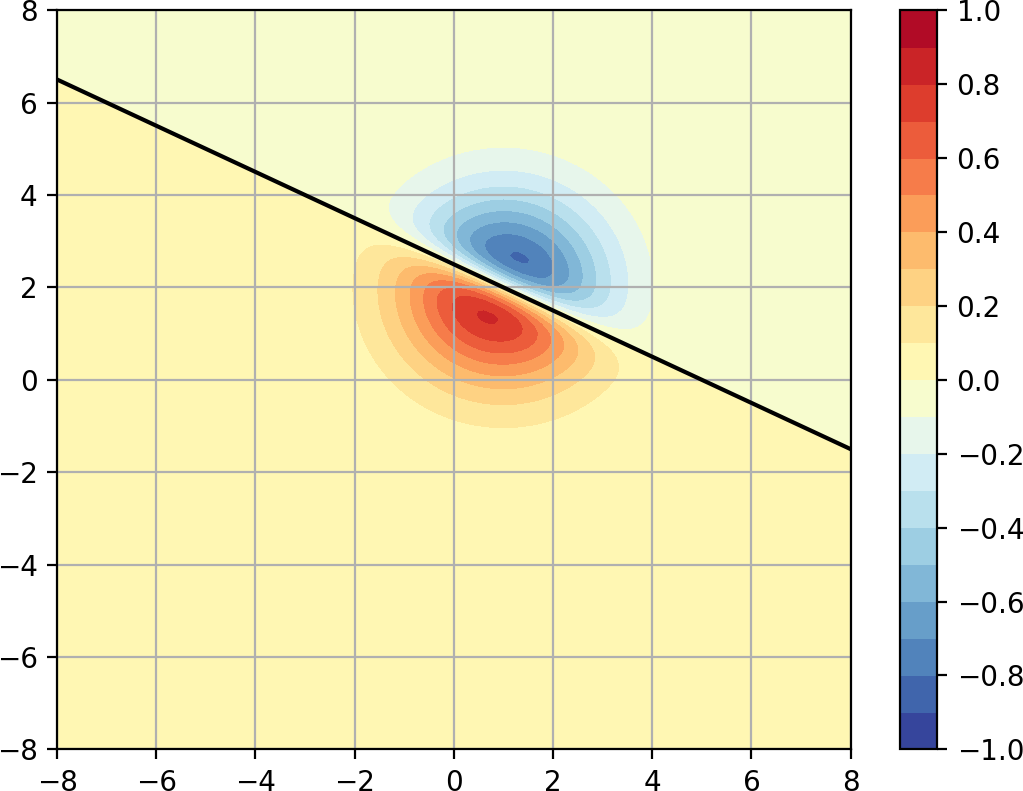
\includegraphics[height=3cm]{images/Matching-behavior/sigma-2-cropped.png}};\pause
        \node (img3)at(img2.north east) [xshift=-0.75cm]{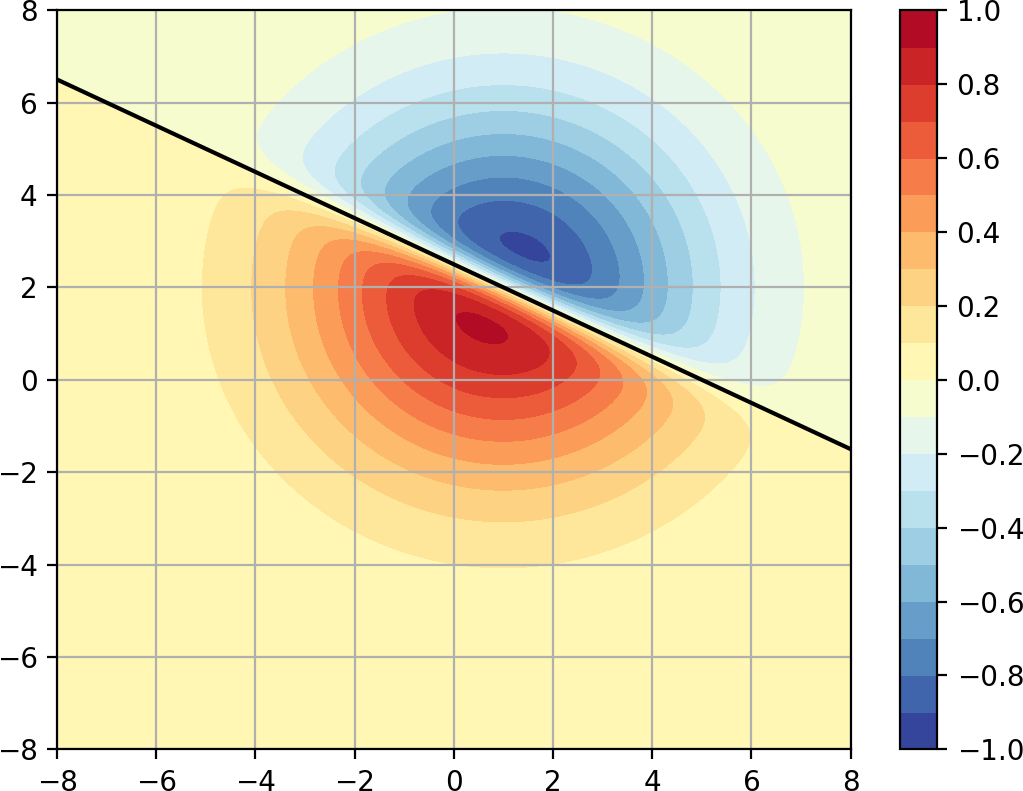
\includegraphics[height=3cm]{images/Matching-behavior/sigma-3-cropped.png}};\pause
        \node (img4)at(img3.south east) [xshift=-0.75cm]{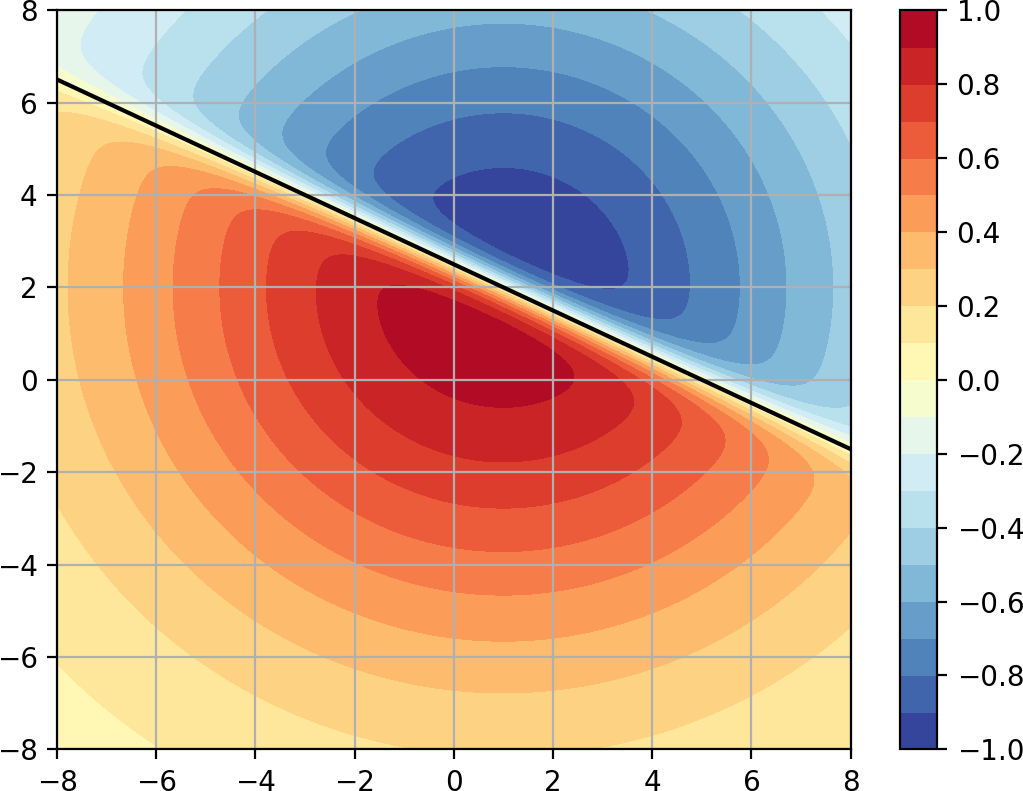
\includegraphics[height=3cm]{images/Matching-behavior/sigma-4-cropped.png}};\pause
        \node (img5)at(img4.north east) [xshift=-0.75cm]{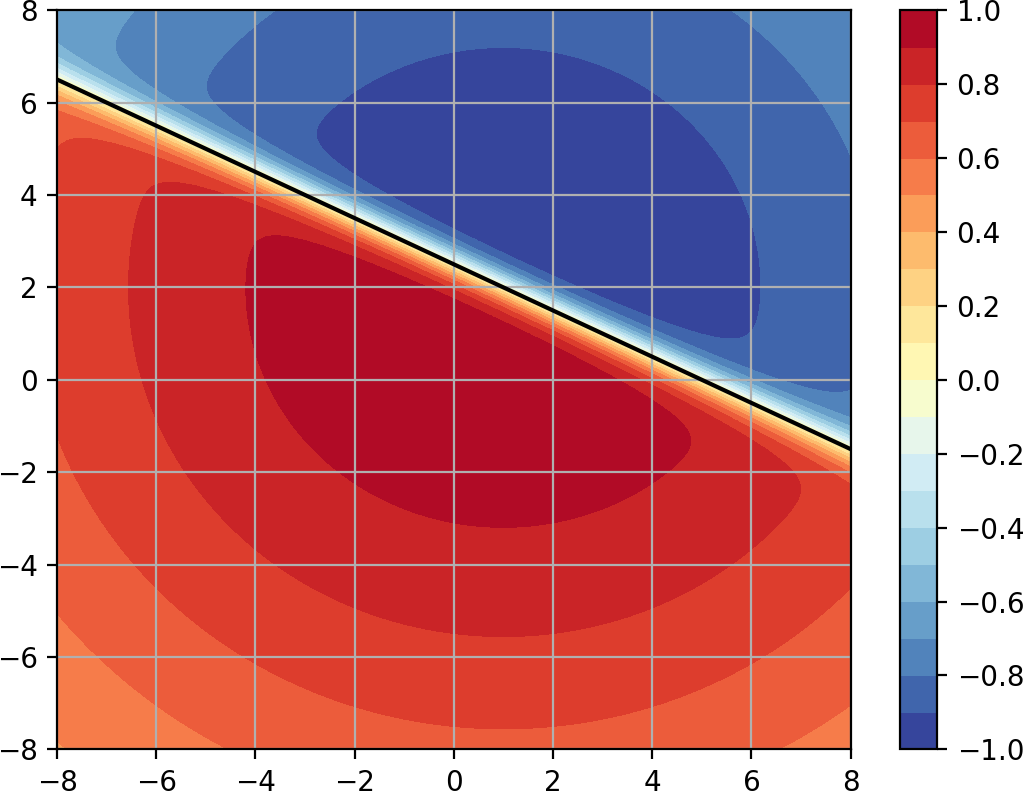
\includegraphics[height=3cm]{images/Matching-behavior/sigma-5-cropped.png}};\pause
        \node (img6)at(img5.south east) [xshift=-0.75cm]{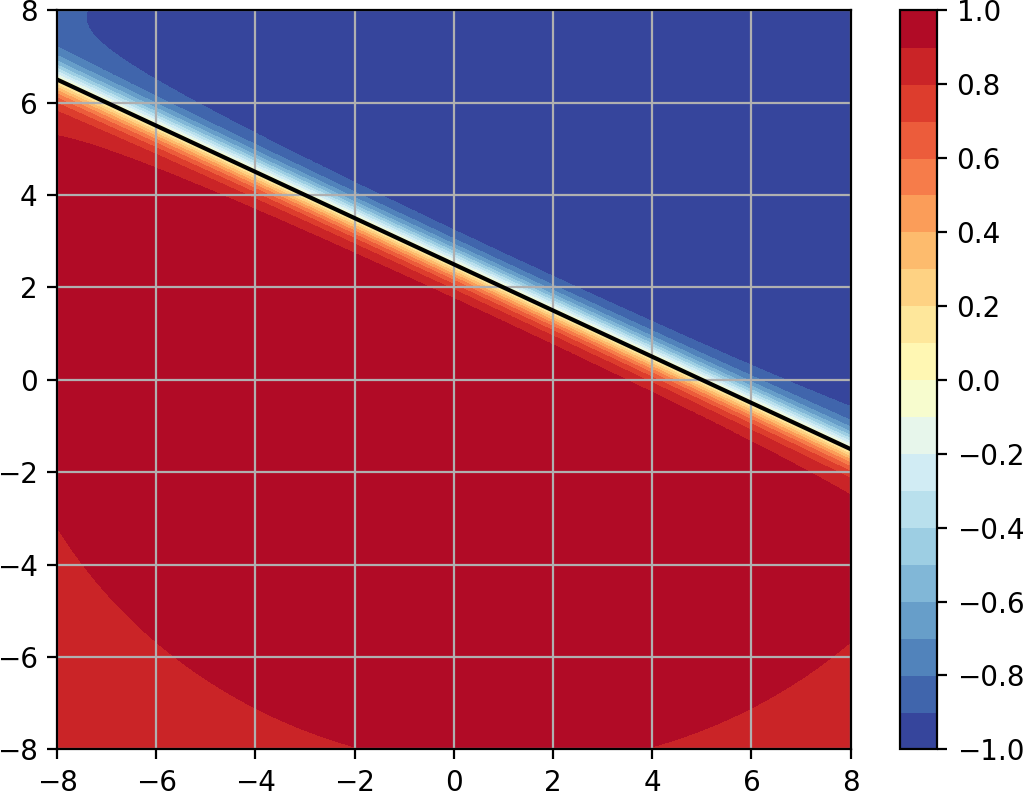
\includegraphics[height=3cm]{images/Matching-behavior/sigma-6-cropped.png}};\pause
        \node (img7)at(img6.north east) [xshift=-0.75cm]{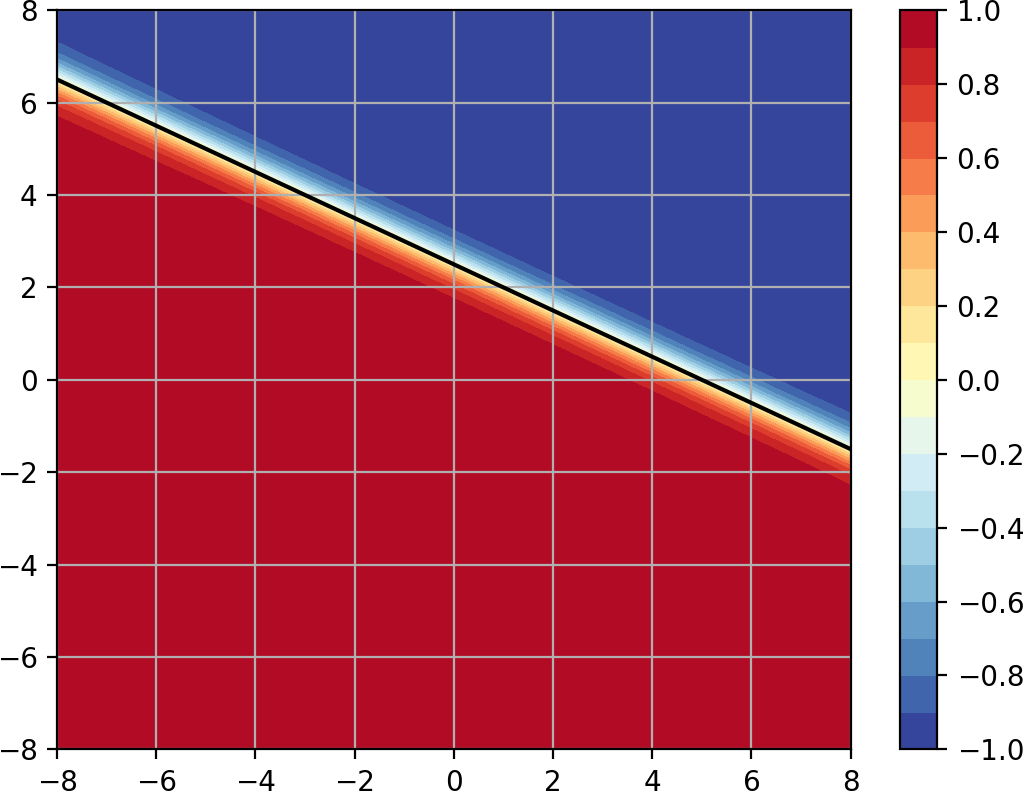
\includegraphics[height=3cm]{images/Matching-behavior/sigma-7-cropped.png}};
    \end{tikzpicture}
\end{frame}

\begin{frame}{Conversion - Initialization of Centers and Variance}
    \begin{block}{Research in Progress}
    Converting a classical neuron to an FGN involves two free parameters: centers $c_i$ and variance $\sigma$.\\
    $\bullet$ Initialize the centers to be the point on the zero line closest to the origin.\\
    $\bullet$ Initialize the variance large enough to not change network behavior.
    \end{block}
    
    \begin{columns}
    \begin{column}{.5\textwidth}
    \begin{figure}
        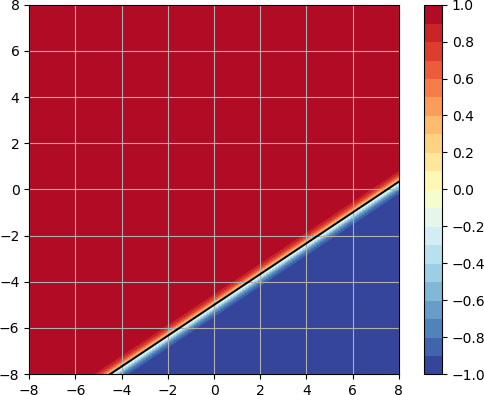
\includegraphics[width=.8\textwidth]{images/2D-Conversion/classic-act.png}
        \caption*{Classic Neuron Activity}
    \end{figure}
    \end{column}
    \begin{column}{.5\textwidth}
    \begin{figure}
        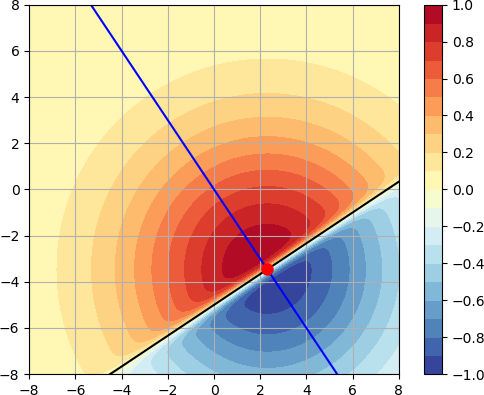
\includegraphics[width=.8\textwidth]{images/2D-Conversion/converted-act.png}
        \caption*{Converted Neuron Finite Activity}
    \end{figure}
    \end{column}
    \end{columns}
    
\end{frame}

\begin{frame}{Training the FGN}
    % talk about adapting SGD to the FGN math
    % adapt the loss function
    \begin{block}{Loss Function - Sigma Regularization}
    $$ \mathcal{L}  = \tilde{\mathcal{L} } + \lambda\sigma^2  $$
    \end{block}
    
    \begin{block}{Gradients for Backpropagation}
    $$ y =  \varphi(\ell)*g = \tanh(\sum_i x_i w_i) * e^{\frac{-1}{\sigma^2}\sum_{i}(x_i-c_i)^2}$$
    \vspace{-0.6cm}
    \begin{align*}
        \text{Weights:\quad} \frac{\partial y}{\partial w_i} &=  x_i \varphi'(\ell) * g  \\[1em]
        \text{Centers:\quad} \frac{\partial y}{\partial c_i} &= \varphi(\ell) * \frac{2(x_i-c_i)}{\sigma^2} * g \\[1em]
        \text{Sigmas:\quad} \frac{\partial y}{\partial \sigma} &= \varphi(\ell) * \frac{2\sum_{i}(x_i-c_i)^2}{\sigma^3}* g
    \end{align*}
    \end{block}
    \end{frame}
    
\begin{frame}{2D Toy Data - Single Neuron Training Sanity Check}
    \begin{columns}
    \begin{column}{.31\textwidth}
        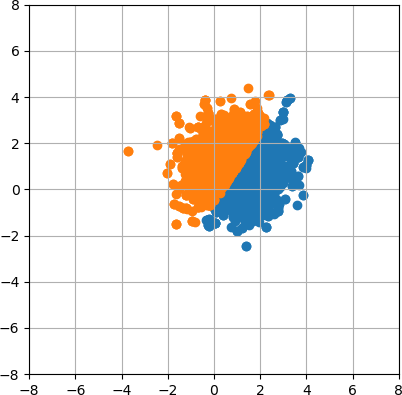
\includegraphics[width=0.85\textwidth]{images/2D-single-neuron/2d-easy-data-cropped.png}\\
        \centering\footnotesize{toy 2D data}\\
        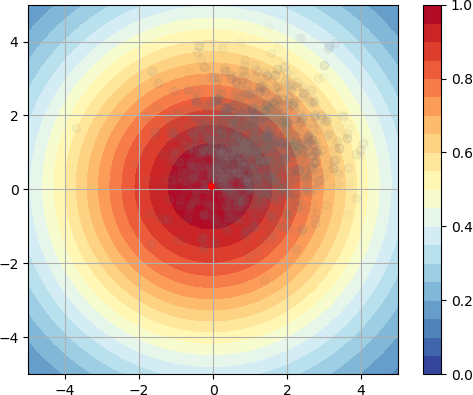
\includegraphics[width=\textwidth]{images/2D-single-neuron/2d-easy-initialg-cropped.png}
        \centering\footnotesize{$g$ pre-training}\\
    \end{column}
    
    \hspace{0.1cm}
    \begin{column}{.31\textwidth}
        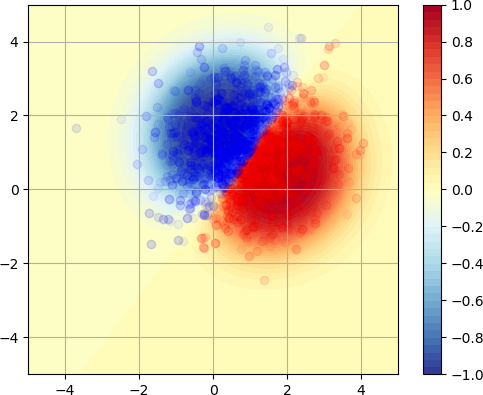
\includegraphics[width=1.02\textwidth]{images/2D-single-neuron/2d-easy-trained-activity-cropped.png}\\
        \centering\footnotesize{activity post-training}\\
        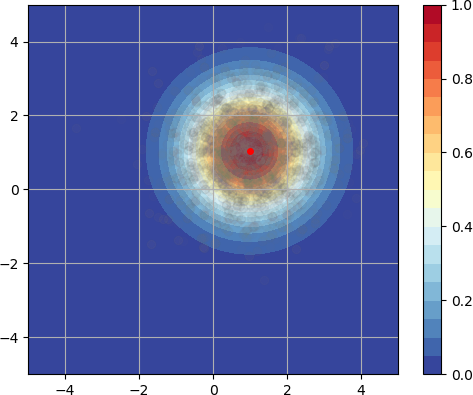
\includegraphics[width=\textwidth]{images/2D-single-neuron/2d-easy-trainedg-cropped.png}\\
         \centering\footnotesize{$g$ post-training}
    \end{column} 
    
    \hspace{0.1cm}
    \begin{column}{.31\textwidth}
        \vspace{0.1cm} \hspace{-0.01cm} 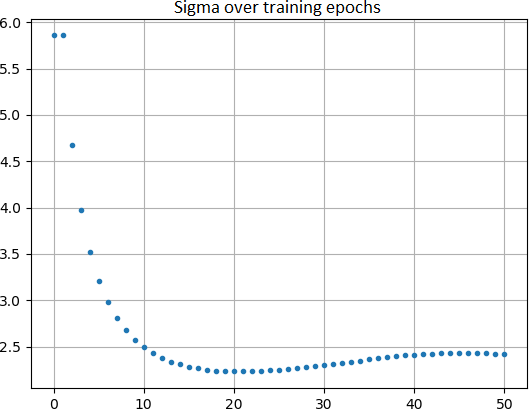
\includegraphics[width=0.84\textwidth,height=3.1cm]{images/2D-single-neuron/2d-easy-sigma-training-cropped.png}\\
        \centering\footnotesize{$\sigma$ over training}\\
        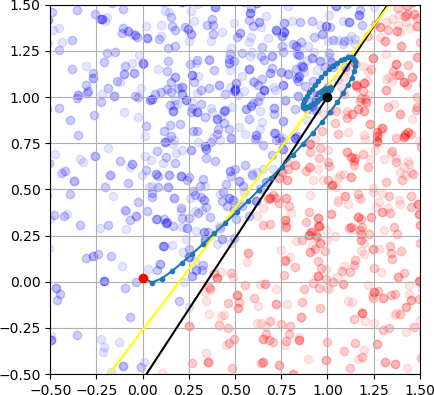
\includegraphics[width=0.92\textwidth]{images/2D-single-neuron/2d-easy-center-path-cropped.png}\\
        \centering\footnotesize{center path}
        
    \end{column}
    \end{columns}

\end{frame}

\begin{frame}{Variants - Different $p$-norms}
    \vspace{-0.3cm}
    \begin{block}{Gaussian Component with $p$-norm}
        $$ g = e^{\frac{-1}{\sigma^2}\lVert x_i-c_i \lVert_p }$$
    \end{block}
    \vspace{0.1cm}
    \centering
    \begin{minipage}{0.87\textwidth}
    \begin{columns}
    \begin{column}{.33\textwidth}
        \raggedright
        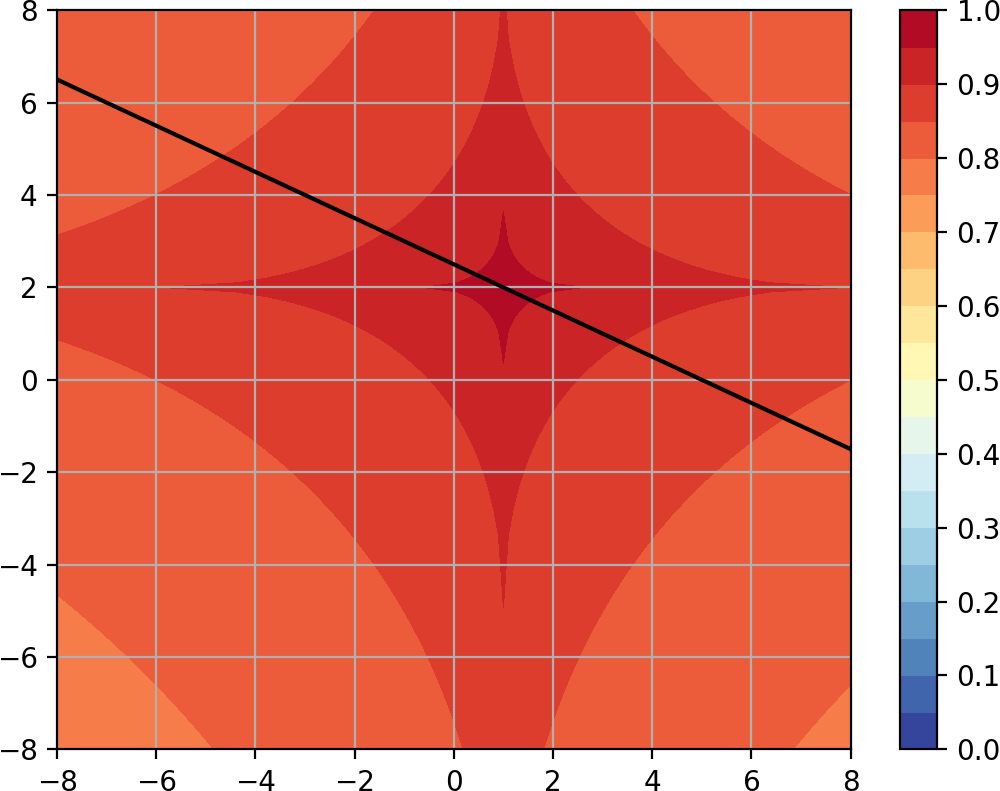
\includegraphics[width=0.98\textwidth]{images/Variants-Norms/ord0.5_g-cropped.png}\\
        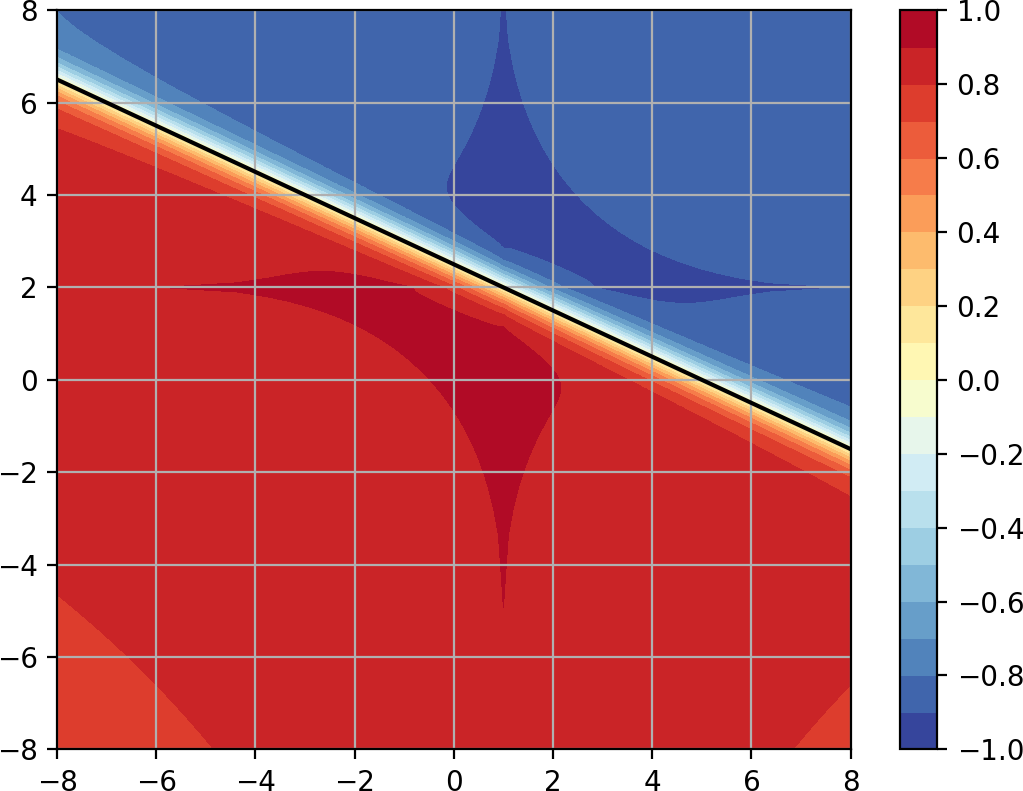
\includegraphics[width=\textwidth]{images/Variants-Norms/ord0.5-cropped.png}\\
        \centering $p=0.5$
    \end{column}
    \begin{column}{.33\textwidth}
        \raggedright
        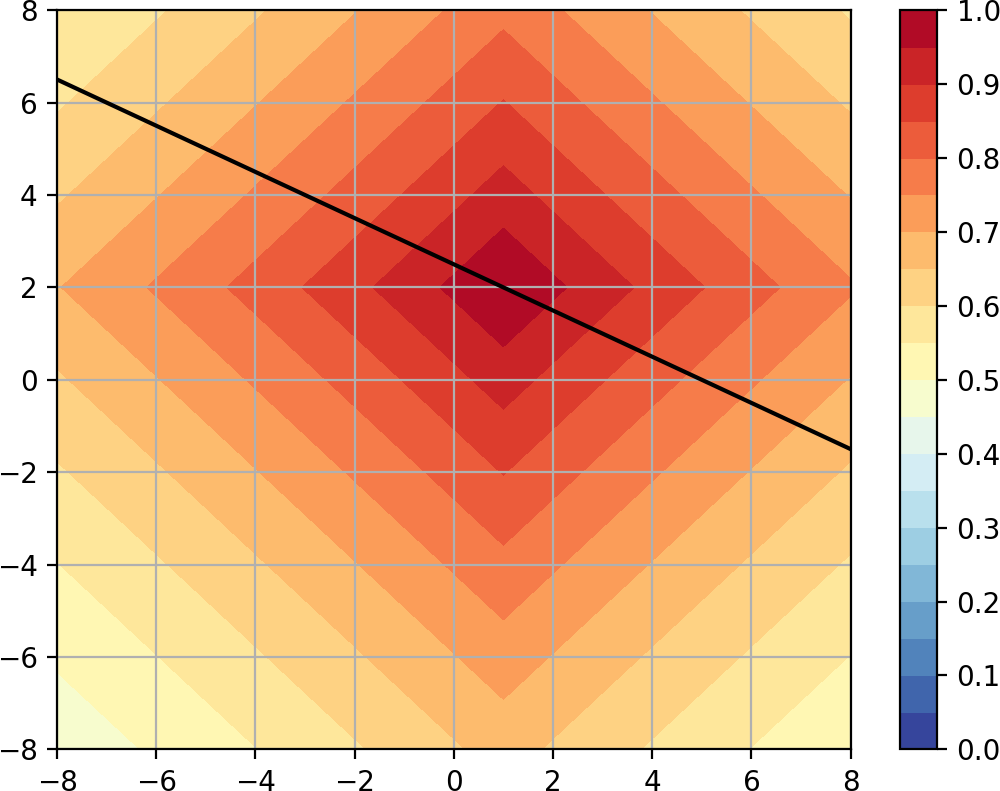
\includegraphics[width=0.98\textwidth]{images/Variants-Norms/ord1_g-cropped.png}\\
        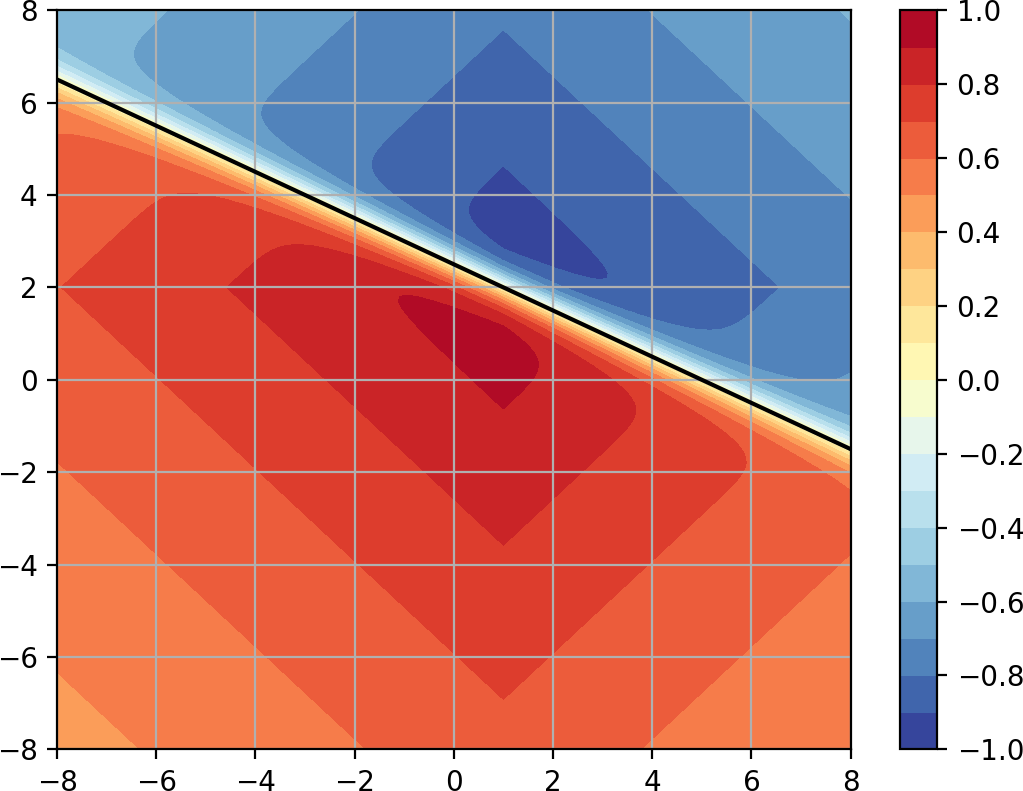
\includegraphics[width=\textwidth]{images/Variants-Norms/ord1-cropped.png}\\
        \centering $p=1$
    \end{column} 
    \begin{column}{.33\textwidth}
        \raggedright
        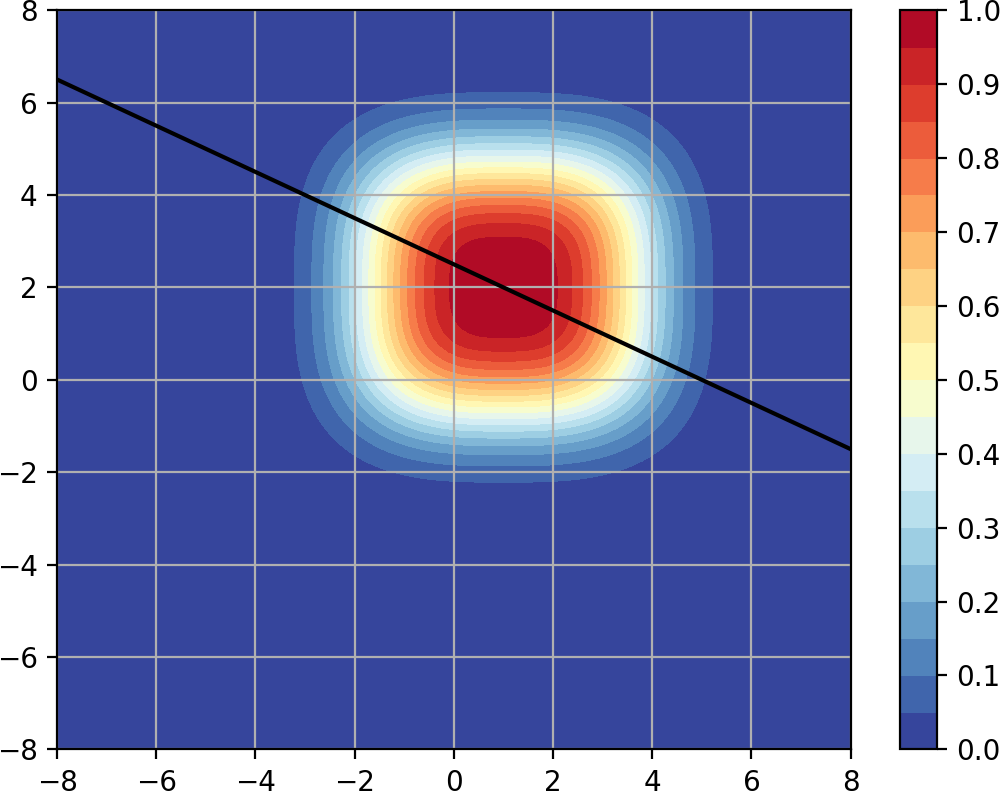
\includegraphics[width=0.98\textwidth]{images/Variants-Norms/ord3_g-cropped.png}\\
        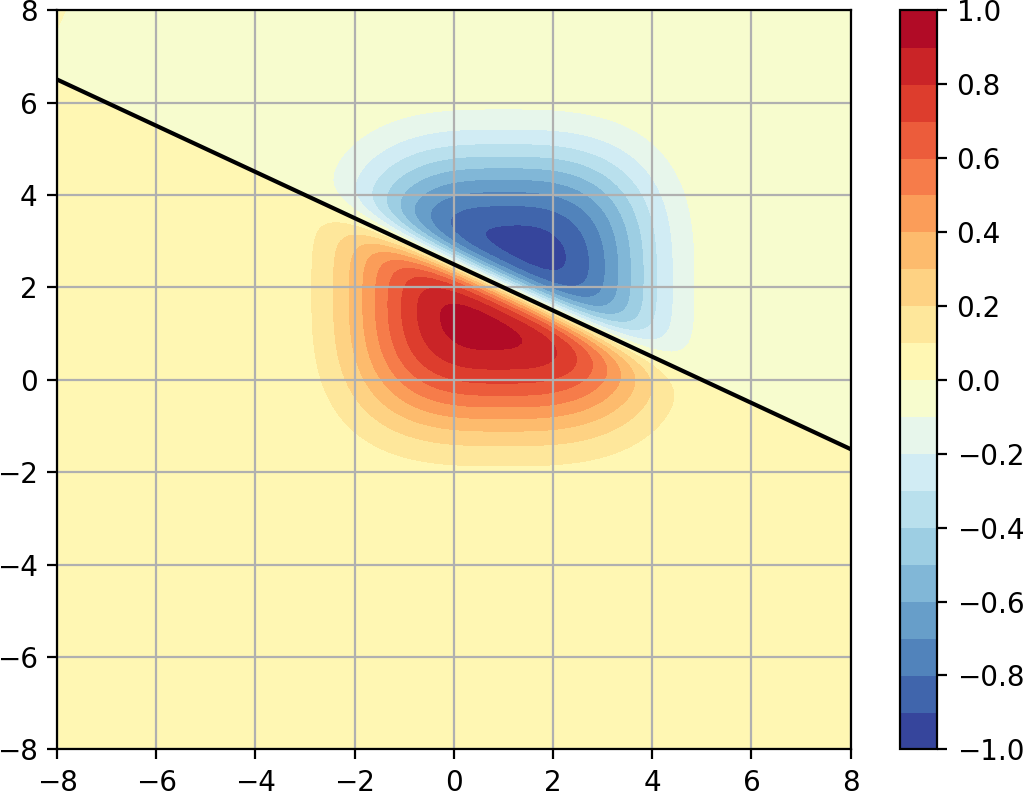
\includegraphics[width=\textwidth]{images/Variants-Norms/ord3-cropped.png}\\
        \centering $p=3$
    \end{column}
    \end{columns}
    \end{minipage}
\end{frame}

\begin{frame}{Variants - Decoupled Bias/Centers}
    \vspace{-0.7cm}
    \begin{block}{}
    The default behavior is to have the bias of the linear term $\ell$ be \emph{unrestricted}: ie: not defined by the centers of the Gaussian term $g$.
    \end{block}
    
    \vspace{0.4cm}
    
    \centering
    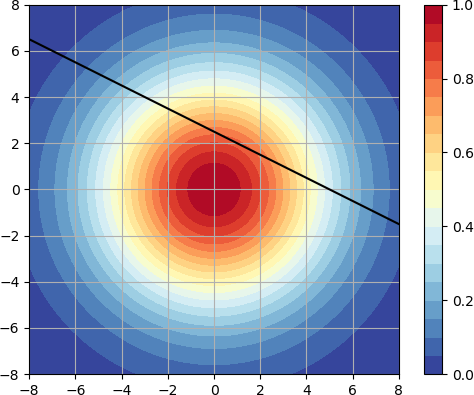
\includegraphics[height=0.5\textheight]{images/2D-Decoupled/var-decoupled-center-g-cropped.png}
    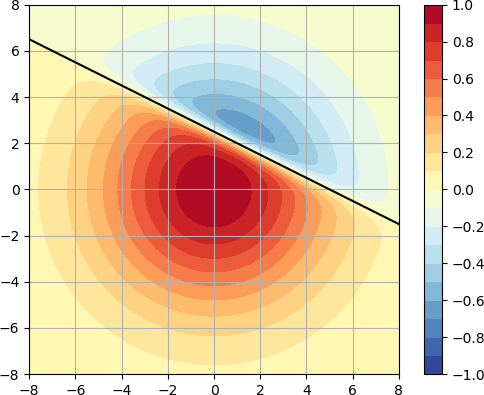
\includegraphics[height=0.5\textheight]{images/2D-Decoupled/var-decoupled-center-activity-cropped.png}\\
    
\end{frame}

\begin{frame}{Variants - Diagonal and Full Covariance}
    \begin{block}{Multivariate Gaussian Component}
    $$ g = e^{-(X-C)^T * \Sigma^{-1} * (X-C)}$$ \\
    with $X=[x_i]$ the inputs vector, $C=[c_i]$ the centers vector and $\Sigma$ the covariance matrix.
    \end{block}
    
    \begin{columns}
    \begin{column}{.5\textwidth}
    \begin{figure}
        \centering
        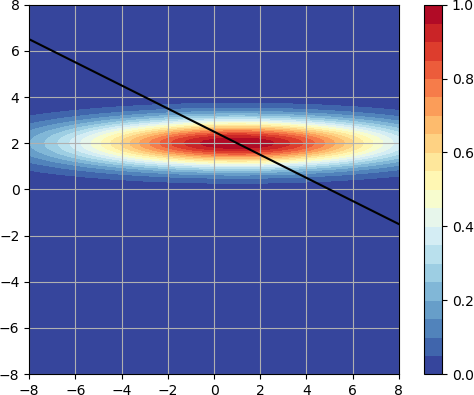
\includegraphics[width=0.81\textwidth]{images/Variants-Diag-Full-Cov/diag_g_activity_cropped.png}
        \caption*{Diagonal $\Sigma$}
    \end{figure}
    \end{column}
     \begin{column}{.5\textwidth}
    \begin{figure}
        \centering
        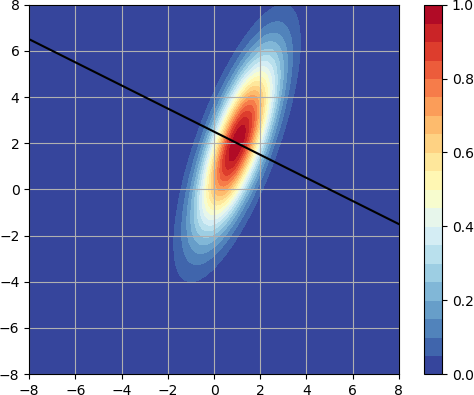
\includegraphics[width=0.81\textwidth]{images/Variants-Diag-Full-Cov/full_g_activity_cropped.png}
        \caption*{Full $\Sigma$}
    \end{figure}
    \end{column}
    \end{columns}
    
\end{frame}


\section{Multi-Layer Finite Gaussian Neural Networks}

\begin{frame}{Multi-Layer Finite Gaussian Neural Networks}
   \begin{block}{Layer $j$ Neuron Outputs}
        $$ y =  \varphi(\ell)*g = \varphi(\sum_i x_{i} w_{i}) * g $$\\[-0.2em]
        $$ g = \max(G_{j-1}) * e^{\frac{-1}{\sigma^2}\sum_{i}(x_i-c_i)^2}$$
        With $x_{i}$ and $G_{j-1}$ the previous layer outputs and Gaussian components.
    \end{block}
    
     \begin{center}
        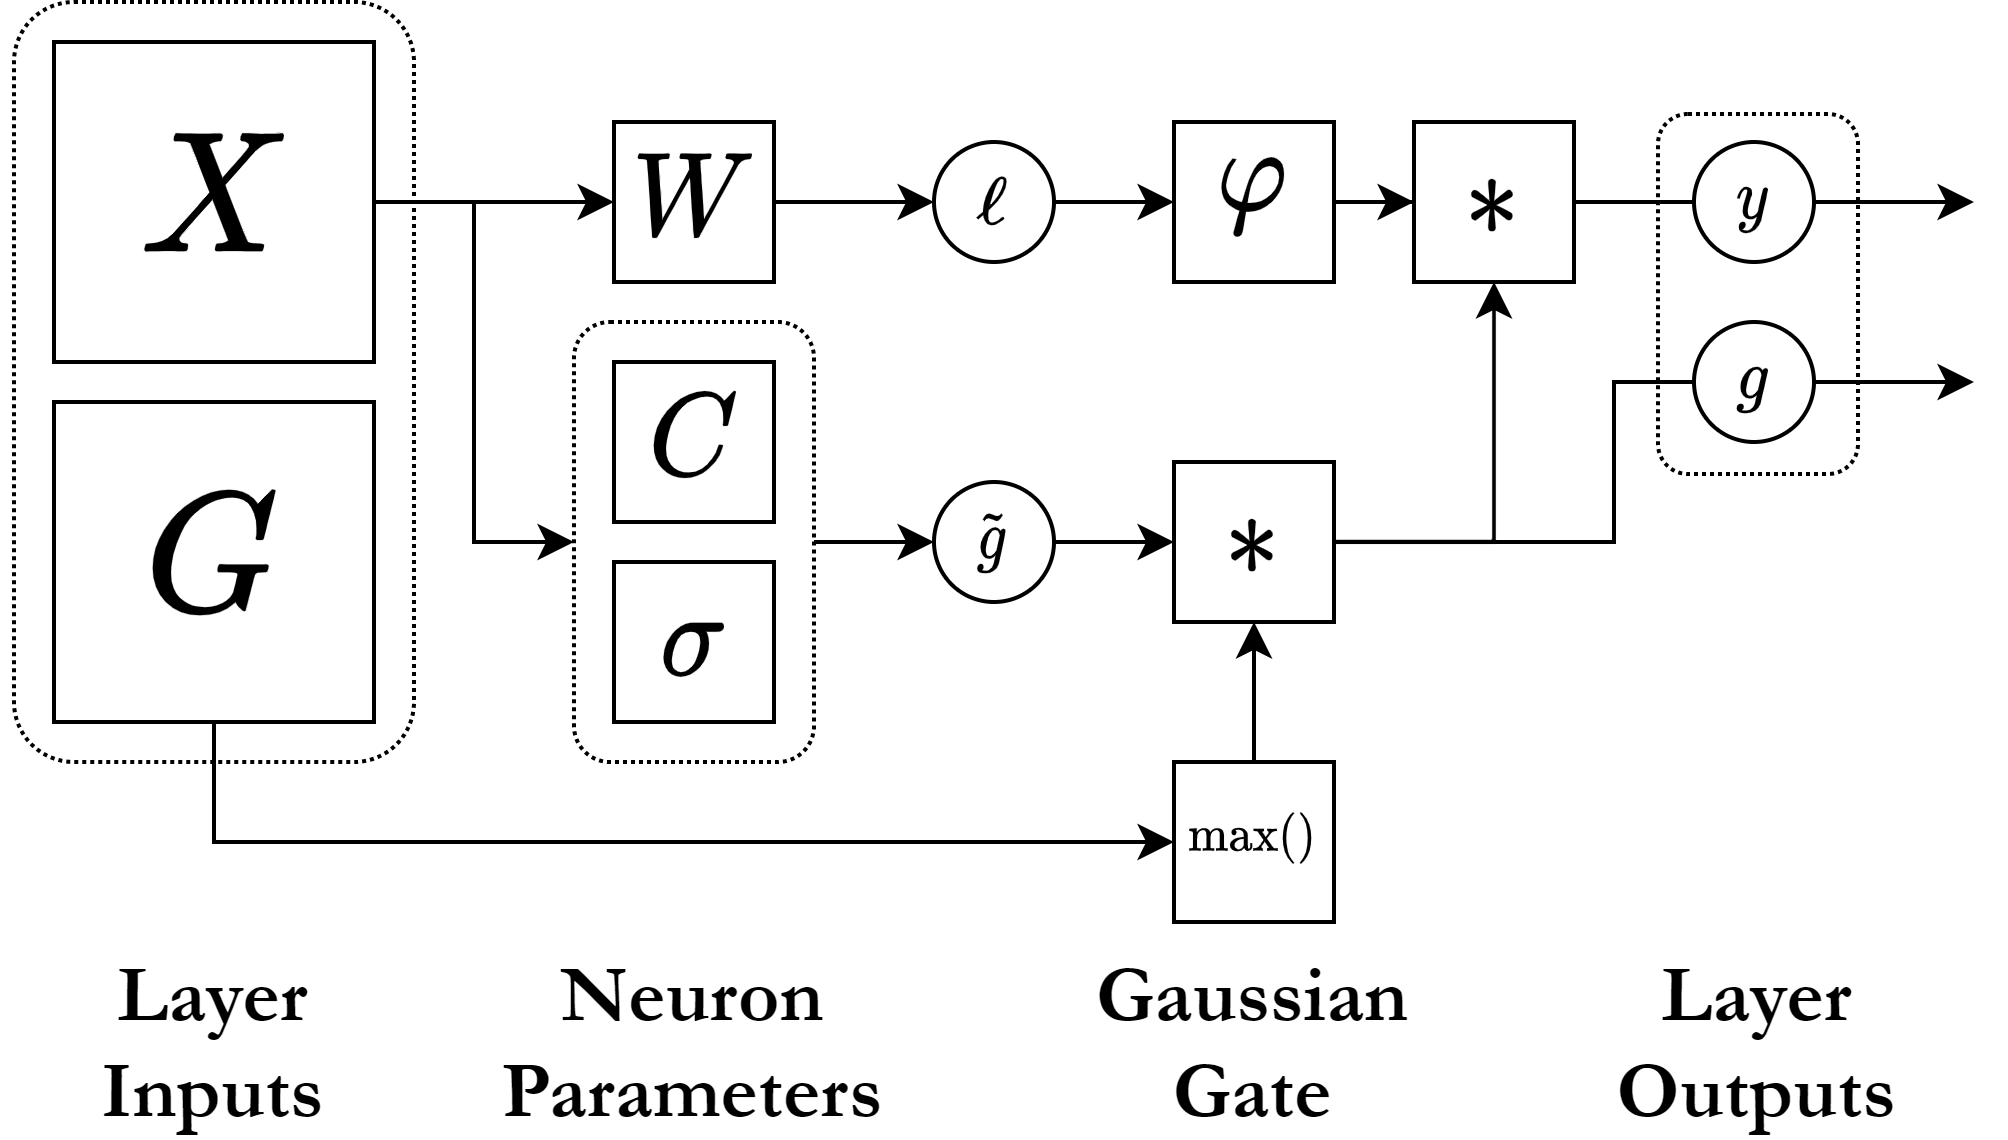
\includegraphics[width=0.6\textwidth]{images/multi-layer-fgn/FGN-Network.png}
    \end{center}

\end{frame}

\begin{frame}{2D Toy Data - Classic vs FGN Network}
    
    \vspace{-1cm}
    \begin{block}{}
    Activity of a classic feedforward network over 2D data, compared to that of an FGN network with the same number of neurons.
    \end{block}

    \begin{columns}
    \begin{column}{.333\textwidth}
    \vspace{2mm}
    \begin{figure}
        \centering
        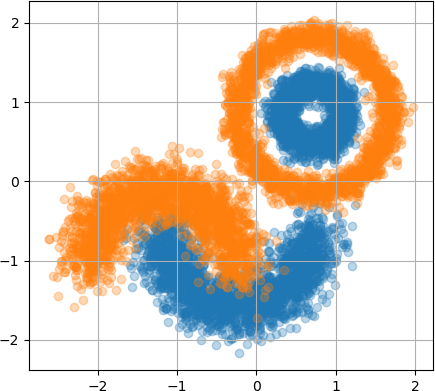
\includegraphics[width=0.92\textwidth]{images/2D-network-toy/2d-toy-data.png}
        \caption*{Toy Data}
    \end{figure}

    \end{column}
    \begin{column}{.333\textwidth}
    \begin{figure}
        \centering
        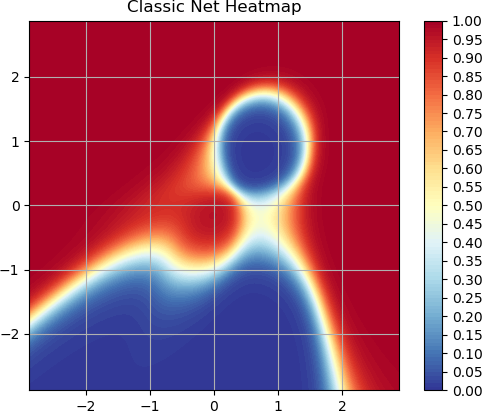
\includegraphics[width=1.\textwidth]{images/2D-network-toy/classic-heatmap.png}
        \caption*{Classic Net Activity}
    \end{figure}
    \end{column}
    \begin{column}{.333\textwidth}
    \begin{figure}
        \centering
        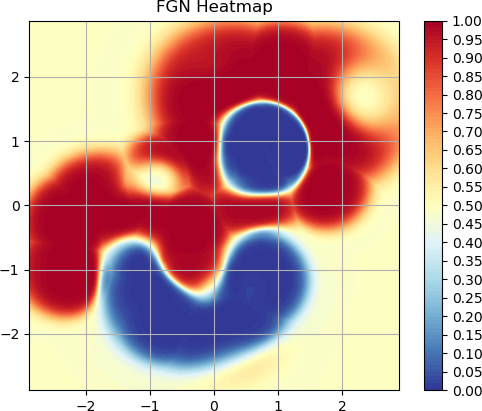
\includegraphics[width=1.\textwidth]{images/2D-network-toy/fgn-heatmap.png}
        \caption*{FGN Net Activity}
    \end{figure}
    \end{column}
    \end{columns}
    
\end{frame}

\begin{frame}{2D Toy Data - Classic vs FGN Network (continued)}
    \vspace{-1cm}
    \begin{block}{}
    Activity of a classic feedforward network over 2D data, compared to that of an FGN network with the same number of neurons (zoomed out).
    \end{block}

    \begin{columns}
    \begin{column}{.333\textwidth}
    \begin{figure}
        \centering
        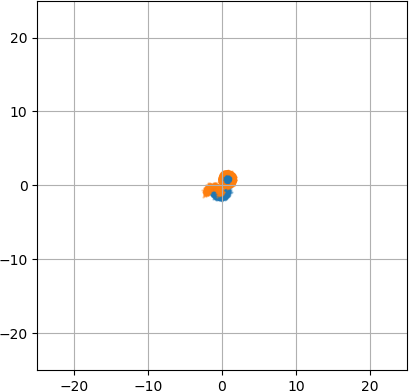
\includegraphics[width=0.92\textwidth]{images/2D-network-toy/2d-toy-data-zoomed-out.png}
        \caption*{Toy Data}
    \end{figure}
    \end{column}
    
    \begin{column}{.333\textwidth}
    \begin{figure}
        \centering
        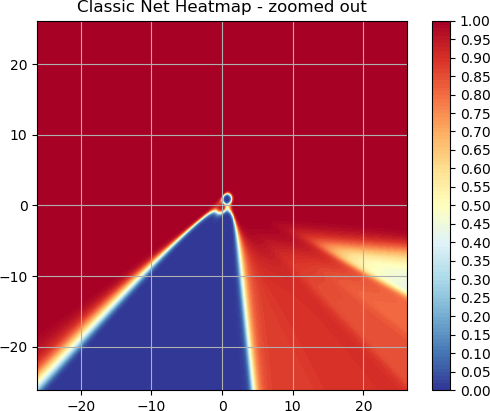
\includegraphics[width=1.\textwidth]{images/2D-network-toy/classic-heatmap-zoomed-out.png}
        \caption*{Classic Net Activity}
    \end{figure}
    \end{column}
    
    \begin{column}{.333\textwidth}
    \begin{figure}
        \centering
        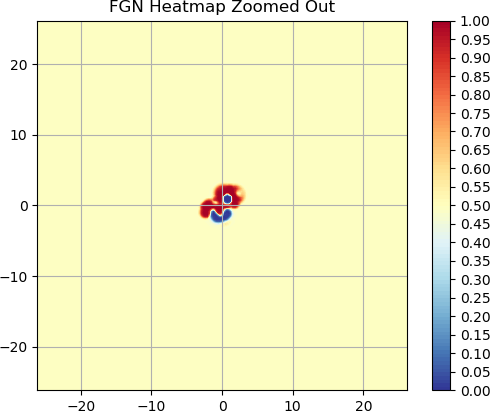
\includegraphics[width=1.\textwidth]{images/2D-network-toy/fgn-heatmap-zoomed-out.png}
        \caption*{FGN Net Activity}
    \end{figure}
    \end{column}
    \end{columns}
    
\end{frame}

\begin{frame}{2D Toy Data - Classic vs FGN Network (addendum)}
    
    \begin{block}{Training Parameters}
    $\bullet$ 32-16 neurons in hidden layers $\bullet$ 1/16 dropout $\bullet$ spherical covariance\\
    $\bullet$ 2-norm $\bullet$ Adam optimizer $\bullet$ cross-entropy loss $\bullet$ 0.001 sigmas loss weight
    \end{block}

    \begin{columns}
    \begin{column}{.333\textwidth}
    \begin{figure}
        \centering
        \includegraphics[width=1.\textwidth]{images/2D-network-toy/centers-init.png}
        \caption*{Initial Centers}
    \end{figure}
    \end{column}
    
    \begin{column}{.333\textwidth}
    \begin{figure}
        \centering
        \includegraphics[width=1.\textwidth]{images/2D-network-toy/training-accuracy.png}
        \caption*{Training Accuracies}
    \end{figure}
    \end{column}
    
    \begin{column}{.333\textwidth}
    \begin{figure}
        \centering
        \includegraphics[width=1.\textwidth]{images/2D-network-toy/sigmas-change.png}
        \caption*{Sigmas Evolution}
    \end{figure}
    \end{column}
    \end{columns}
    
\end{frame}

\begin{frame}{2D Toy Data - Why is the Gaussian Gate Needed?}
    
    \vspace{-1mm}
    
    \begin{block}{}
        Without the Gaussian Gate, activity far from the data defaults to an arbitrary value, not necessarily zero. 
    \end{block}
    
    \begin{columns}
    \begin{column}{.48\textwidth}
    \begin{figure}
        \centering
        \includegraphics[width=1.\textwidth]{images/2D-network-toy/no-gate.png}
    \end{figure}
    \end{column}
    
    \begin{column}{.48\textwidth}
    \begin{figure}
        \centering
        \includegraphics[width=1.\textwidth]{images/2D-network-toy/no-gate-zoomed-out.png}
    \end{figure}
    \end{column}
    \end{columns}

\end{frame}


\section{Networks over MNIST}

\begin{frame}{MNIST and Random Datasets}
    \begin{block}{MNIST Dataset \tiny{(\cite{lecun-mnisthandwrittendigit-2010} LeCun et al.)} }
    $\bullet$ 50K/10K/10K images for train/val/test $\bullet$ 28*28 8bit grayscale pixels\\ 
    \end{block}
    \begin{block}{Random Images Dataset}
    $\bullet$ Fully random pixels (changes mean/variance)\\
    $\bullet$ Shuffled dataset images (preserves mean/variance)\\ 
    \end{block}
    
    \begin{columns}
    \begin{column}{.33\textwidth}
    \begin{figure}
        \centering
        \includegraphics[width=.99\textwidth]{images/mnist-behavior/MNIST-Sample.png}
    \end{figure}
    \end{column}
    \begin{column}{.33\textwidth}
    \begin{figure}
        \centering
        \includegraphics[width=.99\textwidth]{images/mnist-behavior/MNIST-Sample-random-noise.png}
    \end{figure}
    \end{column}
    \begin{column}{.33\textwidth}
    \begin{figure}
        \centering
        \includegraphics[width=.99\textwidth]{images/mnist-behavior/MNIST-Sample-random-shuffled-noise.png}
    \end{figure}
    \end{column}
    \end{columns}
    
\end{frame}

\begin{frame}{Classic Network - MNIST Behavior}
    
    \begin{block}{Classic Feedforward Network Parameters}
    $\bullet$ 64-64 neurons in hidden layers $\bullet$ 0.2 dropout $\bullet$ Train accuracy: 49509/50000 (99\%) $\bullet$ Validation accuracy: 9739/10000 (97\%)
    \end{block}

    \begin{columns}
    \begin{column}{.5\textwidth}
    \begin{figure}
        \centering
        \includegraphics[width=.82\textwidth]{images/mnist-behavior/classic-hist-val.png}
        \caption*{ $>$99\% of confidences $>$0.5}
    \end{figure}
    \end{column}
    \begin{column}{.5\textwidth}
    \begin{figure}
        \raggedright
        \vspace{-3mm}
        \includegraphics[width=.73\textwidth]{images/mnist-behavior/classic-pred-val.png}
        \caption*{}
    \end{figure}
    \end{column}
    \end{columns}
    
    
\end{frame}

\begin{frame}{Classic Network - Fully Random Noise Behavior}

    \begin{columns}
    \begin{column}{.5\textwidth}
    \begin{figure}
        \centering
        \includegraphics[width=.85\textwidth]{images/mnist-behavior/classic-hist-random.png}
        \caption*{ $>$66\% of confidences $>$0.5}
    \end{figure}
    \end{column}
    \begin{column}{.5\textwidth}
    \begin{figure}
        \raggedright
        \vspace{-3mm}
        \includegraphics[width=.73\textwidth]{images/mnist-behavior/classic-pred-random.png}
        \caption*{}
    \end{figure}
    \end{column}
    \end{columns}
    
\end{frame}

\begin{frame}{Classic Network - Shuffled Images Behavior}

    \begin{columns}
    \begin{column}{.5\textwidth}
    \begin{figure}
        \centering
        \includegraphics[width=.82\textwidth]{images/mnist-behavior/classic-hist-shuffled.png}
        \caption*{ $>$78\% of confidences $>$0.5}
    \end{figure}
    \end{column}
    \begin{column}{.5\textwidth}
    \begin{figure}
        \raggedright
        \vspace{-3mm}
        \includegraphics[width=.73\textwidth]{images/mnist-behavior/classic-pred-shuffled.png}
        \caption*{}
    \end{figure}
    \end{column}
    \end{columns}
    
\end{frame}

\begin{frame}{Converted FGN Network - MNIST Behavior}
    
    \begin{block}{Converted FGN Network Parameters}
    $\bullet$ Same architecture as the classic network $\bullet$ $\sigma = 10$\\
    $\bullet$ Same behavior as the classic network over training and validation data.
    \end{block}

    \begin{columns}
    \begin{column}{.5\textwidth}
    \begin{figure}
        \centering
        \includegraphics[width=.82\textwidth]{images/mnist-behavior/converted-hist-val.png}
        \caption*{ $>$99\% of confidences $>$0.5}
    \end{figure}
    \end{column}
    \begin{column}{.5\textwidth}
    \begin{figure}
        \raggedright
        \vspace{-3mm}
        \includegraphics[width=.73\textwidth]{images/mnist-behavior/converted-pred-val.png}
        \caption*{}
    \end{figure}
    \end{column}
    \end{columns}
    
    
\end{frame}

\begin{frame}{Classic vs Converted - MNIST and Random Behavior}

    \vspace{-3mm}
    \begin{columns}
    \begin{column}{.33\textwidth}
    \begin{figure}
        \includegraphics[width=.9\textwidth]{images/mnist-behavior/classic-hist-val.png}
        \centering \tiny{$>$99\% of confidences $>$0.5}
    \end{figure}
    \end{column}
    \begin{column}{.33\textwidth}
    \begin{figure}
        \includegraphics[width=.93\textwidth]{images/mnist-behavior/classic-hist-random.png}
        \centering \tiny{66\% of confidences $>$0.5}
    \end{figure}
    \end{column}
    \begin{column}{.33\textwidth}
    \begin{figure}
        \includegraphics[width=.91\textwidth]{images/mnist-behavior/classic-hist-shuffled.png}
        \centering \tiny{78\% of confidences $>$0.5}
    \end{figure}
    \end{column}
    \end{columns}
    
    \vspace{-3mm}
    \begin{columns}
    \begin{column}{.33\textwidth}
    \begin{figure}
        \includegraphics[width=.9\textwidth]{images/mnist-behavior/converted-hist-val.png}
        \centering \tiny{$>$99\% of confidences $>$0.5}
    \end{figure}
    \end{column}
    \begin{column}{.33\textwidth}
    \begin{figure}
        \includegraphics[width=.91\textwidth]{images/mnist-behavior/converted-hist-random.png}
        \centering \tiny{37\% of confidences $>$0.5}
    \end{figure}
    \end{column}
    \begin{column}{.33\textwidth}
    \begin{figure}
        \centering
        \includegraphics[width=.91\textwidth]{images/mnist-behavior/converted-hist-shuffled.png}
        \centering \tiny{45\% of confidences $>$0.5}
    \end{figure}
    \end{column}
    \end{columns}
    
    
\end{frame}

\begin{frame}{Retrained FGN Network - MNIST Behavior}
    
    \begin{block}{Retrained FGN Network Parameters}
    $\bullet$ Train converted network for \textbf{one} epoch $\bullet$ sigmas loss param $\lambda = 10^{-10}$
    \end{block}

    \begin{columns}
    \begin{column}{.5\textwidth}
    \begin{figure}
        \centering
        \includegraphics[width=.82\textwidth]{images/mnist-behavior/retrained-hist-val.png}
        \caption*{ $>$99\% of confidences $>$0.5}
    \end{figure}
    \end{column}
    \begin{column}{.5\textwidth}
    \begin{figure}
        \raggedright
        \vspace{-3mm}
        \includegraphics[width=.73\textwidth]{images/mnist-behavior/retrained-pred-val.png}
        \caption*{}
    \end{figure}
    \end{column}
    \end{columns}
    
\end{frame}

\begin{frame}{Classic vs Retrained - MNIST and Random Behavior}

    \vspace{-3mm}
    \begin{columns}
    \begin{column}{.33\textwidth}
    \begin{figure}
        \includegraphics[width=.85\textwidth]{images/mnist-behavior/classic-hist-val.png}
        \centering \tiny{$>$99\% of confidences $>$0.5}
    \end{figure}
    \end{column}
    \begin{column}{.33\textwidth}
    \begin{figure}
        \includegraphics[width=.9\textwidth]{images/mnist-behavior/classic-hist-random.png}
        \centering \tiny{66\% of confidences $>$0.5}
    \end{figure}
    \end{column}
    \begin{column}{.33\textwidth}
    \begin{figure}
        \includegraphics[width=.87\textwidth]{images/mnist-behavior/classic-hist-shuffled.png}
        \centering \tiny{78\% of confidences $>$0.5}
    \end{figure}
    \end{column}
    \end{columns}
    
    \vspace{-2mm}
    \begin{columns}
    \begin{column}{.33\textwidth}
    \begin{figure}
        \includegraphics[width=.85\textwidth]{images/mnist-behavior/retrained-hist-val.png}
        \centering \tiny{$>$99\% of confidences $>$0.5}
    \end{figure}
    \end{column}
    \begin{column}{.33\textwidth}
    \begin{figure}
        \includegraphics[width=.85\textwidth]{images/mnist-behavior/retrained-hist-random.png}\\
        \centering \tiny{0.0\% of confidences $>$0.5}
    \end{figure}
    \end{column}
    \begin{column}{.33\textwidth}
    \begin{figure}
        \centering
        \includegraphics[width=.9\textwidth]{images/mnist-behavior/retrained-hist-shuffled.png}
        \centering \tiny{0.05\% of confidences $>$0.5}
    \end{figure}
    \end{column}
    \end{columns}
    
\end{frame}

\begin{frame}{Classic vs FGN - EMNIST Letters \cite{cohen2017emnist}}
 \vspace{-3mm}
    \begin{columns}
    \begin{column}{.33\textwidth}
    \begin{figure}
        \includegraphics[width=.85\textwidth]{images/Letters/hist-classic-letters.png}\\
        \centering \tiny{$>$73\% of confidences $>$0.5}
    \end{figure}
    \end{column}
    \begin{column}{.33\textwidth}
    \begin{figure}
        \includegraphics[width=.85\textwidth]{images/Letters/hist-converted-letters.png}\\
        \centering \tiny{42\% of confidences $>$0.5}
    \end{figure}
    \end{column}
    \begin{column}{.33\textwidth}
    \begin{figure}
        \includegraphics[width=.85\textwidth]{images/Letters/hist-retrained-letters.png}\\
        \centering \tiny{0.0\% of confidences $>$0.5}
    \end{figure}
    \end{column}
    \end{columns}
    
    \vspace{-2mm}
    \begin{columns}
    \begin{column}{.33\textwidth}
    \begin{figure}
        \includegraphics[width=.85\textwidth]{images/Letters/classic-letters.png}
    \end{figure}
    \end{column}
    \begin{column}{.33\textwidth}
    \begin{figure}
        \includegraphics[width=.85\textwidth]{images/Letters/converted-letters.png}
    \end{figure}
    \end{column}
    \begin{column}{.33\textwidth}
    \begin{figure}
        \centering
        \includegraphics[width=.85\textwidth]{images/Letters/retrained-letters.png}
    \end{figure}
    \end{column}
    \end{columns}
    
\end{frame}


\begin{frame}{Checkpoint}
\textcolor{gray}{My works aims to:}
\begin{itemize}
    \item \textcolor{gray}{make it easy to convert existing models to the FGN architecture}
    \item \textcolor{gray}{while preserving the existing model's behavior on real data}
    \item and offering resistance against some adversarial attacks.
\end{itemize}
    
\end{frame}


\begin{frame}{Successful Attacks Comparison}
    \begin{block}{}
        Successful Attack: $\bullet$ changes the class $\bullet$ confidence above 0.5
    \end{block}
    \begin{figure}
        \centering
        \includegraphics[width=.88\textheight]{images/successful-attacks-comparisons/succesful_fgsm_count.png}
    \end{figure}
\end{frame}

\begin{frame}{Successful Attacks Comparison (continued)}
   \begin{tikzpicture}
        \node (img1) {\includegraphics[height=3.7cm]{images/successful-attacks-comparisons/fgsm-comp-0.png}};\pause
        \node (img2)at(img1.south east) [xshift=-1.2cm][yshift=-0.8cm]{\includegraphics[height=3.7cm]{images/successful-attacks-comparisons/fgsm-comp-1.png}};\pause
        \node (img3)at(img2.north east) [xshift=-1.2cm][yshift=0.8cm]{\includegraphics[height=3.7cm]{images/successful-attacks-comparisons/fgsm-comp-2.png}};\pause
        \node (img4)at(img3.south east) [xshift=-1.2cm][yshift=-0.8cm]{\includegraphics[height=3.7cm]{images/successful-attacks-comparisons/fgsm-comp-3.png}};\pause
        \node (img5)at(img4.north east) [xshift=-1.2cm][yshift=0.8cm]{\includegraphics[height=3.7cm]{images/successful-attacks-comparisons/fgsm-comp-4.png}};
    \end{tikzpicture}
\end{frame}


\begin{frame}{Observations - FGSM Boundaries}

    \centering{Starting from an image, where does the FGSM adversarial example land?}
   \begin{tikzpicture}
        \node (img1){\includegraphics[width=0.6\textwidth]{images/observations/classic-bounds.png}};\pause
        \node (img2)at(img1.center)[xshift=0cm]{\includegraphics[width=0.6\textwidth]{images/observations/converted-bounds.png}};\pause
        \node (img3)at(img2.center)[xshift=0cm]{\includegraphics[width=0.64\textwidth]{images/observations/long-bounds.png}};
    \end{tikzpicture}
    
\end{frame}

\begin{frame}{Observations - Space in between Images}

    \centering{What the space in between two images look like?}
   \begin{tikzpicture}
        \node (img1){\includegraphics[width=0.6\textwidth]{images/observations/classic-img8toimg4.png}};\pause
        \node (img2)at(img1.center)[xshift=0cm]{\includegraphics[width=0.6\textwidth]{images/observations/converted-img8toimg4.png}};\pause
        \node (img3)at(img2.center)[xshift=0cm]{\includegraphics[width=0.64\textwidth]{images/observations/long-img8toimg4.png}};
    \end{tikzpicture}
    
\end{frame}

\section{Remaining Work}
\begin{frame}{Remaining Work}

    Currently Finite Gaussian Neurons:
    \begin{itemize}
        \item \textcolor{gray}{make it easy to convert existing models to the FGN architecture}
        \item \textcolor{gray}{while preserving the existing model's behavior on real data}
        \item \textcolor{gray}{and offering resistance against some adversarial attacks.} 
    \end{itemize}
    ~

    To further validate the usefulness of Finite Gaussian Neurons, I want to:
    \begin{itemize}
        \item implement a finite Gaussian version of the convolutional layer,
        \item test against PGD and Carlini-Wagner attacks,
        \item test the transferability of examples,
        \item and expanding to CIFAR-10 and SPEECHCOMMANDS tasks.
    \end{itemize}
    All while continuing to explore their properties and best practices, and comparing to other research.
\end{frame}

\begin{frame}{Convolutional Layer}
% Popularized in 2012 with Alexnet on Imagenet.
\begin{figure}
    \centering
    \includegraphics[width=.85\textwidth]{images/image net.png}
    \caption*{Alexnet by \cite{krizhevsky2012imagenet} \fullcite{krizhevsky2012imagenet}}
\end{figure}
\end{frame}

\begin{frame}{Projected Gradient Descent and Carlini-Wagner Attack}
    \begin{block}{PGD Attack: Iterated FGSM}
    \centering $x^{t+1} = \Pi_{x+S}(x^t + \epsilon(\text{sign}(\nabla_x L(\Theta, x, y)  ))$
    \end{block}

    \begin{block}{Carlini-Wagner Attack}
    Given $x,t$, search for $w$ that solves:
    \begin{center}{minimize $||\frac{1}{2}(\text{tanh}(w)+1) -x||_2^2 + c \cdot f(\frac{1}{2}(\text{tanh}(w)+1) $} \end{center}
    with $f$ defined as:
    \begin{center}{$f(x') = \text{max}(\text{max}\{Z(x')_i : i\neq t\} - Z(x')_t, -K)$} \end{center}
    \cite{carlini2017evaluating} \fullcite{carlini2017evaluating}
    \end{block}
\end{frame}

\begin{frame}{Transferability of Examples}
    
    Test Finite Gaussian Networks against:
    \begin{itemize}
        \item adversarial examples generated using another model,
        \item and universal perturbations (\cite{moosavidezfooli2017universal} Moosavi-Dezfooli et al.)
    \end{itemize}
    
\end{frame}


\begin{frame}{CIFAR-10 and SPEECHCOMMANDS}
    \begin{block}{ CIFAR-10 \tiny{(\cite{Krizhevsky2009LearningML} Krizhevsky et al.)} }
    $\bullet$ 60K Images $\bullet$ 32*32 color images $\bullet$ 10 classes
    \end{block}
    \begin{figure}
        \includegraphics[width=0.66\textwidth]{images/cifar10.png}
    \end{figure}
    
    \begin{block}{SPEECHCOMMANDS \tiny{(\cite{DBLP:journals/corr/abs-1804-03209} Pete Warden)} }
    $\bullet$ 65K one-second long utterances $\bullet$ 30 short words\\
    $\bullet$ single channel $\bullet$ thousands of different speakers
    \end{block}
    \begin{figure}
        \includegraphics[width=0.36\textwidth]{images/yes.jpg}
        \caption*{\emph{yes}}
    \end{figure}
    
\end{frame}

\begin{frame}{Properties, Best Practices, and Other Research}
    % prop 1: empty space in between classes? what are those filaments
    % make the derivative of the centers not rely on good/bad classification
    % best practice: init of size, centers, impact of p-norm?

    \begin{block}{Properties}
    \begin{itemize}
        \item What is going on in spaces in between classes?
        \item Can the training of centers be made independent of classification?
    \end{itemize}
    \end{block}
    
    \begin{block}{Best Practices}
    \begin{itemize}
        \item How to initialize the sizes and centers of FGNs?
        \item When to retrain models and for how long?
        \item Do the variants (p-norms, covariance matrix) help in any way?
    \end{itemize}
    \end{block}
    
    \begin{block}{Comparison to Other Research}
    \begin{itemize}
        \item Bayesian Neural Networks (\cite{mullachery2018bayesian} Mullachery et al. 2018)
        % Ensembles are not resistant to adversarial examples.
        \item Training Speed: \emph{Fast is Better Than Free} \cite{wong2020fast} by Wong et al.
    \end{itemize}
    
    \end{block}
    
\end{frame}


\begin{frame}{Open Source}
    
    \begin{block}{}
    All the code is available at:\\
    \quad $\bullet$ \url{https://github.com/grezesf/FGN---Research}.\\
    ~\\
    It includes:\\
    \quad $\bullet$ library of functions to implement your own FGNs or convert existing networks to FGNs.\\
    \quad $\bullet$ all the notebooks used to run experiments, analyse results, and generate the figures.
    % TODO have a notebook open and ready to run (the sanity check one)

    \end{block}
    \centering
    \includegraphics[width=.08\textheight]{images/misc/GitHub-Mark.png} 
    \includegraphics[width=.4\textheight]{images/misc/gpl3.PNG}

\end{frame}


\begin{frame}[allowframebreaks]{Citations}
    \printbibliography

\end{frame}


\end{document}